\documentclass[12pt]{report}
\usepackage{../Style/WUbiblio,../Style/WUthesis}
\usepackage[latin1]{inputenc}
\usepackage{amsmath}
\usepackage{amsfonts}
\usepackage{amssymb} 
\usepackage{graphicx}
\usepackage{siunitx}
\usepackage{tikz}
\usepackage{pgfplots}
\usepackage[mode = buildnew]{standalone}
%\usepackage{hyperref}
\usepackage{marvosym}
\usepackage{url}
\usepackage{pdfpages}

\DeclareSIUnit\gauss{G}
\usetikzlibrary{decorations.pathmorphing}
\pgfplotsset{compat=1.7}

\begin{document}

%%%%%%%%%%%%%%%%%%%%%%%%%%%%%%%%%%%%%%%%%%%%%%%%%%
% Title
%%%%%%%%%%%%%%%%%%%%%%%%%%%%%%%%%%%%%%%%%%%%%%%%%%
\title{Improving Laser Guide Stars through Magnetic Resonant Pulsing}
\author{Adam Newton Wright}
\thesissupervisor{Dr. Michaela Kleinert}

\includepdf[pages=1-2]{../ApkerSummary/AWrightApkerSummary.pdf}
\newpage

\maketitle

\newpage

%%%%%%%%%%%%%%%%%%%%%%%%%%%%%%%%%%%%%%%%%%%%%%%%%%
% Summary
%%%%%%%%%%%%%%%%%%%%%%%%%%%%%%%%%%%%%%%%%%%%%%%%%%
%\noindent\textbf{\Huge Summary}\\






%%%%%%%%%%%%%%%%%%%%%%%%%%%%%%%%%%%%%%%%%%%%%%%%%%
% Presentations
%%%%%%%%%%%%%%%%%%%%%%%%%%%%%%%%%%%%%%%%%%%%%%%%%%
\begin{center}
\textbf{Presentations and Publications}\\
\end{center}

\begin{description}
\item Adam N. Wright, \textit{Increasing Laser Guide Star Fluorescence through Magnetic Resonant Pulsing}, Senior Symposium, Linfield College, April 2018\\
	
\item Adam N. Wright, \textit{Improving Laser Guide Stars through Magnetic Resonant Pulsing}, Senior Theses, Student Scholarship Recognition Day, Willamette University, April 2018\\

\item Adam N. Wright, \textit{Increasing Atomic Fluorescence: Magnetic Resonant Pulsing}, Poster Session, Institute of Optics, University of Arizona, January 2018\\
	
\item Adam N. Wright, \textit{Improving Laser Guide Stars through Magnetic Resonant Pulsing}, Senior Thesis Presentation I, Willamette University, December 2017\\

\item Adam N. Wright, \textit{Focus Recovery in Computational Microscopy}, Research Experience for Undergraduates, University of Rochester, August 2017\\

\item Adam N. Wright, \textit{Improving Laser Guide Stars through Magnetic Resonant Pulsing}, Senior Thesis Proposal, Willamette University, May 2017\\

\item Donald Swen, Adam N. Wright, \textit{Construction, Calibration, and Application of Dye Lasers}, Student Scholarship Recognition Day, Willamette University, April 2017\\


\end{description}





%%%%%%%%%%%%%%%%%%%%%%%%%%%%%%%%%%%%%%%%%%%%%%%%%%
% Acknowledgements
%%%%%%%%%%%%%%%%%%%%%%%%%%%%%%%%%%%%%%%%%%%%%%%%%%
\begin{acknowledgments}
I would like to acknowledge and thank the following people and organizations for the help and support they have given me and this project:

\begin{description}
   \item Dr. Michaela Kleinert, for her support as an academic and laboratory advisor. She is an amazing professor and mentor with an extraordinary ability to teach, mentor, and advise. I am incredibly grateful for the opportunity to work and learn under her.
   \item Dr. Jed Rembold, for his help with Vim, LaTex, and Python. He has given me a passion for most things computing, and has inspired many projects and helped me when those projects became riddled with bugs. 
   \item Luke Galbraith Russell, for his friendship. He has helped me stay passionate about physics, encouraged me when I was stressed out, spent long nights doing homework with me, and went to the gym with me the next morning at 6 am. 
   \item All of my lab partners, everyone in the Kleinert Lab, and the Physics cohort. You all are so awesome, helpful, and encouraging!
   \item The Physics Department professors: Dr. Daniel Borrero, Dr. Rick Watkins, Dr. David Altman, and Dr. Roberta Bigelow. You all are incredible wizards and have taught me everything I know.
   \item The National Science Foundation, for their financial support.
   \item Dr. Scott Bergeson from Brigham Young University, for his collaboration and support.
\end{description}


\end{acknowledgments}





%%%%%%%%%%%%%%%%%%%%%%%%%%%%%%%%%%%%%%%%%%%%%%%%%%
% Abstract
%%%%%%%%%%%%%%%%%%%%%%%%%%%%%%%%%%%%%%%%%%%%%%%%%%
\begin{abstract}

%\section*{General Abstract}
%
%\noindent Modern astronomy relies on the ability to take extremely high resolution images of distant celestial objects, such as stars and galaxies. However, in order to obtain such high resolution images, astronomers must use a combination of laser guide stars --- artificial stars created by shining laser light into the upper atmosphere where it is reflected back to earth by atoms --- and computer algorithms to restore distorted images. In this thesis, we look at improving the brightness of laser guide stars by using a laser that emits bursts of light instead of a continuous beam of light. We build this proposed laser, model magnetic field conditions, and measure the brightness of our experimental laser guide star, showing that pulsed lasers indeed create brighter laser guide stars, especially for locations near the equator where the geomagnetic field is perpendicular to the laser beam.
%
%
%\section*{Technical Abstract}

\noindent Atoms with a magnetic moment residing in a magnetic field experience Larmor precession, a precession of the atom's total atomic angular momentum due to the torque the magnetic field exerts on the atom, with frequency known as the Larmor frequency. This precession degrades the benefits obtained through optical pumping, a technique used to increase atomic fluorescence, through a nonoptimal redistribution of the atom's angular momentum. However, according to Kane et al. (2014), a technique known as magnetic resonant pulsing suggests that laser light pulsed at the Larmor frequency can mitigate this degradation and increase atomic fluorescence by reestablishing the benefits of optical pumping. We test this technique by constructing a pulsed laser and measuring the fluorescence of rubidium confined in a magnetic field. We report a 32\% increase in fluorescence between CW and pulsed laser light when the laser beam is perpendicular to the magnetic field. This method can significantly increase the irradiance of laser guide stars due to the near-equatorial position of many telescopes, giving angles between their laser beams and the geomagnetic field of nearly $90 ^{\circ}$.

\end{abstract}


\tableofcontents
%\listoftables
\listoffigures

\pagebreak


%%%%%%%%%%%%%%%%%%%%%%%%%%%%%%%%%%%%%%%%%%%%%%%%%%
% Introduction
%%%%%%%%%%%%%%%%%%%%%%%%%%%%%%%%%%%%%%%%%%%%%%%%%%
%%%%%%%%%%%%%%%%%%%%%%%%%%%%%%%%%%%%%%%%%%%%%%%%%%
% Part: Introduction
% Filename: intro.tex
% Created: September 9, 2017
% Author: Adam Wright
%%%%%%%%%%%%%%%%%%%%%%%%%%%%%%%%%%%%%%%%%%%%%%%%%%


%%%%%%%%%%%%%%%%%%%%%%%%%%%%%%%%%%%%%%%%%%%%%%%%%%
% Introduction
%%%%%%%%%%%%%%%%%%%%%%%%%%%%%%%%%%%%%%%%%%%%%%%%%%

\chapter{Introduction}
In 1609, Galileo Galilei pointed a device made of two lenses at the sky and saw for the first time tiny craters on the moon, small objects orbiting Jupiter, and even the phases of Venus \cite{nasa,keckhistory}. With observations from this crude contraption, Galileo experimentally showed that Venus was orbiting the Sun. This evidence supported the theoretical model of a heliocentric solar system, proposed in the sixteenth century by Nicolaus Copernicus and expounded upon by Johannes Kepler in the seventeenth century \cite{copern}. As time progressed, inquisitive minds began to wonder what else could be discovered with the power of magnification. Telescopes, as they would be coined, began a rapid period of advancement. Lenses were made larger in diameter in order to collect more light and thus view fainter objects. Optical components were fabricated with less imperfection, allowing for better resolution. As the laws of optics were understood more clearly, the curvature and indices of refraction of lenses were exploited, and achromatic, aspheric, and cylindrical lenses were created, ridding telescopes of significant aberrations. Mirrors were created with surface deviations of less than \SI{1}{\angstrom} \cite{daewook}, resulting in reflecting telescopes of amazing purity. By the late twentieth century, telescopes were as optically perfect as they could be. No advances in optics would allow them to see with greater resolution. However, there was a lingering problem: \textit{atmospheric distortion}.

Atmospheric distortion is caused by the inhomogeneity of Earth's atmosphere. As light from astronomical bodies passes through the atmosphere, the varying levels of pressure, density, and temperature cause small distortions in the image of that object. In order to rid data of atmospheric distortions, astronomers image distant point sources, e.g. natural stars, to calculate the distortion that the atmosphere is imposing on entering light. This distortion is then sent to a deformable mirror, which is able to form a conjugate wavefront that can effectively negate the atmospheric distortion. The image of the astronomical body is then reflected off this deformable mirror, and the resulting image is free of atmospheric distortion. This technique is known as \textit{adaptive optics} and is an image processing problem, not an  optical component problem. (See Appendix B for more information on adaptive optics.)

In order for adaptive optics systems to work, there must be a bright enough star in the sky. Using a natural star, however, has severe limitations, namely that there is not always a star within the field of view, and even so, that star may not be bright enough. Thus,  artificial guide stars, known as laser guide stars and shown in Fig. \ref{fig:lgs2}, are often created. A laser guide star is formed in the upper atmosphere by interacting laser light with sodium atoms that were deposited there by meteors as they burn up in Earth's atmosphere \cite{Kibblewhite2009}. They are preferred over natural stars due to their ability to be spatially placed into the telescope's field of view, their brightness, and their well known spectral emission.\footnote{Furthermore, clusters of laser guide stars can be created, as shown in Fig. \ref{fig:lgs2}, which can eliminate more optical aberrations, such as the cone effect (focus anisoplanatism) \cite{multiplelgs}.} Since the resolution of a telescope depends upon its adaptive optics system, and the adaptive optics system in turn depends upon the guide star, it is important to know how laser guide stars work and how they can be improved. 

\begin{figure}[t]
		\centering
		%\begin{minipage}{.45\textwidth}
		%\includegraphics[width=0.9\linewidth]{Images/lgs2.jpg}
		%\end{minipage}
		%\begin{minipage}{.45\textwidth}
		\includegraphics[width = .8\textwidth]{Images/lgsinsky.jpg}
		%\end{minipage}
		\caption{Long exposure of a laser guide star created by the Gemini Observatory as seen in the night sky \protect\cite{gemini}.}
		%\caption{Laser guide star shone into the night sky at ESO's Very Large Telescope \protect\cite{lgs2} (left) and a time lapse of a laser guide star as seen in the sky \protect\cite{gemini}.}
		\label{fig:lgs2}
\end{figure}

One important property of laser guide stars is their brightness, which can be increased by improving the intensity of the laser beam, increasing the size of the laser beam, or by using various optical techniques to increase the atom's probability of absorbing and emitting photons. Nevertheless, there remain ``the three evils'' of laser guide stars, each of which decreases brightness: Larmor precession, recoil, and transition saturation (i.e. depumping). Larmor precession, depicted in Fig. \ref{fig:larpre}, is the precession of the atom's total atomic angular momentum vector about the axis of the magnetic field. It arises in atoms that possess a magnetic moment, and thus experience a torque in a magnetic field. This phenomenon decreases the benefits obtained from optical pumping through a nonoptimal redistribution of the atom's angular momentum vector. The second ``evil,'' recoil, is due to the spontaneous emission of photons, which causes the atom to gain velocity in order to conserve momentum. Due to the Doppler effect, a redshift occurs, rendering the atom unable to absorb more laser light. The third ``evil,'' transition saturation, is the depopulation of atoms from a higher ground state to a lower ground state, resulting in a different wavelength for absorption \cite{Holzlohner2012}. We focus on mitigating the effects of Larmor precession, but will also briefly consider transition saturation.

\begin{figure}[h]
		\centering
		\begin{tikzpicture}
			\node at (0,0) {\includegraphics[scale = .5]{Images/larmorprecession.png}};
			\node at (1,1) {$\vec \mu$};
			\node at (0,3.5) {$\vec B$};
			\node at (1.5,2.5) {$\omega$};
		\end{tikzpicture}
		\caption{Schematic of an atom with an angular momentum vector $\vec \mu$ precessing about a magnetic field $\vec B$ with angular speed $\omega$ \protect\cite{larmor}.}
		\label{fig:larpre}
\end{figure}


In 2014, Kane et al. proposed a technique to improve laser guide stars, which they coined \textit{magnetic resonant pulsing} (MRP) \cite{Kane2014}. This technique proposes using a pulsed laser beam with a repetition rate equal to atom's the Larmor frequency, the frequency of the atom's precession in the magnetic field. For sodium in the Earth's magnetic field, these frequencies are typically around \SI{200}{\kilo Hz} to \SI{400}{\kilo Hz}. MRP has been computationally simulated by Rampy et al. and Kane et al. \cite{Rampy2010,Kane2014}. Their data show that lasers pulsed at the Larmor frequency of the atom in a magnetic field increase photon return when compared with continuous wave light as the direction of the laser beam nears perpendicular to the magnetic field.

In this thesis, we experimentally test MRP under controlled conditions. We investigate the construction of a magnetic resonant pulsed laser through both a short-cavity dye laser pumped by a frequency-doubled $\text{Nd:YVO}_4$ and a diode laser chopped with an acousto-optic modulator (AOM). Although laser guide stars involve laser light interacting with sodium, we use rubidium since it is similar to sodium (including a similar gyromagnetic ratio, magnetic moment, and Larmor frequency, in addition to both being alkali metals), but because it is also the overall focus of this laboratory. Fluorescence measurements are taken of rubidium atoms confined in an absorption cell and surrounded by a variable magnetic field. 


Since the Larmor precession of an atom depends linearly on the strength of the magnetic field, we are able to change the frequency of the atom's precession to any frequency within the range of $\SI{200}{\kilo \hertz}$ to $\SI{2000}{\kilo \hertz}$ by changing the strength of the magnetic field. Thus, we can bring the system into and out of magnetic resonant pulsing by adjusting the strength of the magnetic field while measuring the amount of light the atoms absorb and emit. By changing the orientation of the magnetic fields with respect to the laser beam, we are able to test the dependence of fluorescence upon the angle between the magnetic field and the laser beam. 

In Chapter 2, we outline the atomic and quantum theory that underpins laser guide stars and the details of magnetic resonant pulsing. In Chapter 3, we detail the experimental laser system with wavelength on resonance with rubidium and pulsed at the Larmor frequency. Chapter 4 describes the magnetic field configuration used. In Chapter 5, we detail the final experimental setup, show how measurements were made, and present the results of the fluorescence measurements. Chapter 6 concludes this thesis, presents problems encountered, and provides an outlook for future experiments.




%%%%%%%%%%%%%%%%%%%%%%%%%%%%%%%%%%%%%%%%%%%%%%%%%%
% Background
%%%%%%%%%%%%%%%%%%%%%%%%%%%%%%%%%%%%%%%%%%%%%%%%%%
%%%%%%%%%%%%%%%%%%%%%%%%%%%%%%%%%%%%%%%%%%%%%%%%%
% Adam Wright
% Background
% back.tex
%%%%%%%%%%%%%%%%%%%%%%%%%%%%%%%%%%%%%%%%%%%%%%%%%%

\chapter{Background}
Laser guide stars (LGS)\footnote{LGS will refer to both the plural and singular of the word, e.g. ``LGS are frequently used in modern astronomy'' and ``LGS systems consist of many components.'' Context should provide the correct form throughout reading this thesis.}  are invaluable instruments in modern astronomy, allowing observations of extremely high resolution to be made even in unfavorable atmospheric conditions. An important quality of an LGS is its brightness, which affects the overall performance of the adaptive optics system and limits the resolution that the telescope can achieve. However, taking advantage of the atoms' precession in a magnetic field, the brightness of LGS can be increased through magnetic resonant pulsing (MRP). In this chapter, we describe the quantum theory behind LGS and magnetic resonant pulsing.


\section{Quantum Theory of Laser Guide Stars}

Atoms can be thought of being composed of two parts: the nucleus, or the core of the atom, and electrons, smaller charged particles surrounding the nucleus. In a simple model, the electrons in the atom are ``orbiting'' the nucleus. This model, proposed by Niels Bohr in the early twentieth century, is known as the \textit{Bohr Model}. The electrons orbit in discrete radii of quantized energy, or shells, each of which is denoted by the principal quantum number $n = 1,2,3,\dots$. Each electron shell refers to a certain energy of the atom, and electrons are free to transition between shells as long as energy is conserved during this transition.\footnote{Other quantities, such as angular momentum, must also be conserved. These will be addressed shortly.} As a pedagogical example, we can calculate the energy needed for an electron transitioning between shells in hydrogen using the famous Rydberg formula

\begin{equation}
  \Delta E = hc R_H\left( \frac{1}{n_f^2} - \frac{1}{n_i^2}\right),
  \label{rydberg}
\end{equation}
%
where $h$ is Planck's constant, $c$ is the speed of light in a vacuum, $R_H = \SI{1.1e7}{\per\meter}$ is the Rydberg constant for hydrogen, $n_f$ is the principal quantum number of the final state, and $n_i$ is the principal quantum number of the initial state. Empirically, we see that atoms emit photons (i.e. particles of light) when they decay from states of higher energy to those with lower energy. Furthermore, the energy of these emitted photons is exactly equal to the energy difference between these two states. Knowing that the energy of a photon is

\begin{equation}
  E = h f = \frac{hc}{\lambda},
  \label{energyfrequency}
\end{equation}
%
where $f$ is the frequency of the photon, and $\lambda$ is the wavelength of the photon, we can calculate the wavelength of light a transition would emit using this and Eq. \ref{rydberg},


\begin{equation}
		\frac{1}{\lambda} = R\left( \frac{1}{n_f^2} - \frac{1}{n_i^2}\right).
  \label{rydbergw}
\end{equation}
%
Thus, if we wanted to know the wavelength of a photon that is emitted when an electron in the $n_i=1$ shell is completely ejected from the atom (ionization), we could compute this by letting $n_f = \infty$ and find that $\lambda_{L_{\infty}} = $ \SI{91}{\nano \meter} (this one transition in the well known Lyman series \cite{Townsend}). This process is also reversible, meaning an atom can be excited by absorbing a photon of wavelength equal to this calculated wavelength. The wavelength of light needed for this excitation is known as the resonant wavelength. This is the foundation of LGS --- laser light resonant with sodium is shone onto sodium atoms in the atmosphere, the atoms absorb light, and then emit this light in random directions, creating a ``globe'' of light (see Appendix A for a discussion of laser guide stars).


The Bohr model, however, is not accurate, especially for atoms of more than one electron. In order to fully describe the physics of the atoms, \textit{quantum mechanics}, the branch of physics that concerns itself with describing the behavior of particles and energies of the smallest scales, is needed. The fundamental equation in quantum mechanics is the Schr\"{o}dinger equation, which details how a quantum system will evolve and is given by

\begin{equation}
	i \hbar \frac{\partial}{\partial t} \left| \psi(\vec r,t) \right> = \hat H \left| \psi (\vec r,t)\right>,
	\label{eq:schrodingers}
\end{equation}
%
where $i = \sqrt{-1}$, $\hbar = \frac{h}{ 2 \pi}$ is the reduced Planck's constant, $\psi (\vec r,t)$ is the spatially and temporally dependent wavefunction of the particle, and $\hat H$ is the Hamiltonian operator, describing the energy of the system. For a particle in a time-independent system with a central potential dependent upon $r$, the wave function $\psi (\vec r)$ can be separated into three functions each of which describes a particular coordinate 

\begin{equation}
	\psi(r, \theta, \phi) = R(r) \Theta(\theta) \Phi(\phi), 
	\label{eq:seppsi}
\end{equation}
%
where $R(r)$ is the radial function, $\Theta(\theta)$ is the polar function, and $\Phi(\phi)$ is azimuthal function.\footnote{It is common for $\Theta$ and $\Phi$ to be combined into one function, which can be written in terms of the spherical harmonics $Y^m _L$ described by the quantum numbers $L$ and $m_L$ \cite{Townsend}.} Substituting Eq. \ref{eq:seppsi} into Eq. \ref{eq:schrodingers}, the spatial functions $R(r)$, $\Theta(\theta)$, and $\Phi(\phi)$ can each be solved separately. In order to solve them, however, three quantum numbers are introduced: the principal quantum number $n$ (introduced earlier), coming from the radial function of the Schr\"{o}dinger equation; the orbital angular momentum quantum number $L$, coming from the polar function; and the magnetic quantum number $m_L$, coming from the azimuthal function.


It was later realized\footnote{Spin was empirically discovered through the famous Stern-Gerlach experiment in 1922 where silver atoms were deflected by an inhomogeneous magnetic field depending on their spin \cite{Townsend}.} that a fourth quantum number, known as spin and denoted $S$, was needed in order to fully describe the behavior of many particles. Spin describes a particle's intrinsic (spin) angular momentum and takes on full or half integer values of the reduced Planck's constant $\hbar$. For example, electrons are spin-$\frac{1}{2}$ particles and thus have a $z$-component of spin $S_z = \pm \frac{\hbar}{2}$, while photons are spin-$1$ particles with $S_z = \pm \hbar$. 

When all of these quantum numbers are considered collectively, we find interesting phenomena occurring in the energies of atoms. Upon first inspection, we see that many energy levels actually consist of multiple, closely-spaced sublevels. These sublevels are caused in part by the relativistic energy of the particles and in part by the interaction between the electron's spin and its orbital angular momentum. Spin, being a value of the intrinsic angular momentum, can couple with the \textit{orbital} angular momentum, causing an interaction that shifts and splits each energy level. The relativistic energy simply shifts the value of the energy level by more accurately describing the particle's kinetic energy. Collectively, these corrections are known as the \textit{fine structure} \cite{Kibblewhite2009}. The spin-orbit coupling follows the formula 

\begin{equation}
  \vec J = \vec L + \vec S,
  \label{fineequation}
\end{equation}
%
where $\vec J$ is the total angular momentum vector, $\vec L$ is the orbital angular momentum vector with magnitude $|\vec L| = \hbar \sqrt{L (L + 1)}$, and $\vec S$ is the spin angular momentum vector with magnitude $|\vec S| = \hbar \sqrt{S(S+1)}$. The values that the splitting can thus take are $|J| = |L - S|, \dots, |L +S|$ in integer steps. Thus, for a state of $L=0$ with a particle of spin-$\frac{1}{2}$, $J = |0-\frac{1}{2}|, \dots, |0+\frac{1}{2}| = \frac{1}{2}$, indicating there being only an energy shift and not split. However, for the $L=1$ state, $J = |1-\frac{1}{2}|,\dots, |1+\frac{1}{2}| = |-\frac{1}{2}|, \dots, |\frac{3}{2}| =  \frac{1}{2}, \frac{3}{2}$, indicating a two--fold split.


We can look even more carefully at the energy levels of atoms. We saw how the spin $\vec S$ interacted with the orbital angular momentum $\vec L$ to cause an energy split, but the total angular momentum $\vec J$ can also interact with the spin of the nucleus, causing yet another, even smaller\footnote{For hydrogen, these shifts are on the order of millionths of an electronvolt \cite{feynman}. Compared with the ionization energy of $13.6 \text{ eV}$, this is quite small.} splitting of the energy levels. This is the \textit{hyperfine structure} and follows the formula

\begin{equation}
\vec F = \vec J + \vec I,
  \label{hyperfine}
\end{equation}
%
where $\vec F$ is the new total angular momentum vector and $\vec I$ is the nuclear spin.\footnote{This splitting holds true for atoms with relatively low atomic number, including the atoms we are studying (rubidium and sodium). Heavier atoms couple differently.} The splitting obeys $F = |J-I|, \dots, |J+I|$, causing degeneracy for all states with $J \neq 0$ and $I \neq 0$.

Finally, if we consider the atom to be in a magnetic field, we observe another splitting known as the \textit{Zeeman effect}. The Zeeman effect results from a magnetic field interacting with $\vec F$, causing a precession of this vector about the axis of the magnetic field. The energy shift follows the equation

\begin{equation}
  \Delta E = \mu_B m_F g_F B,
  \label{zeeman}
\end{equation}
%
where $\mu_B$ is the Bohr magneton, $m_F$ is the $z$-component of the total angular momentum, $g_F$ is the Land\'{e} $g$-factor,\footnote{The Land\'{e} $g$-factor is a particular g-factor (a dimensionless number describing the magnetic moment) that accounts for both the spin and orbital angular momentum of the particle. It is described mathematically as 
  \begin{equation}
	g_F = g_J \frac{F(F+1) -I(I+1) + J(J+1)}{2F(F+1)} + g_I \frac{F(F+1) + I(I+1) -J(J+1)}{2F(F+1)},
	\label{lande}
  \end{equation}
%
where $g_{J,I}$ are the Lande g-factors for the those particular quantum values, and $F,J,I$ are the quantum values discussed earlier.} and $B$ is the magnetic field. The splitting is quantized by the values of the $z$-component of the orbital angular momentum, $m_F = -F, \dots, F$. Since sodium, the basis of LGS systems, lives within the geomagnetic field and has a magnetic moment, its energy levels are split due to the Zeeman effect.

Bringing everything together, we can show these energy shifts and splits schematically, as in Fig. \ref{fig:energysplitting} for the case of $I = 3/2$. From left to right, the order of magnitude of the splitting gets smaller. The scale of the fine structure splitting is $Z \alpha^2$, where $Z$ is the atomic number and $\alpha = 1/137$ is the fine structure constant \cite{feynman}. The scale of the hyperfine structure is typically an order of magnitude smaller than the fine structure, and the Zeeman split is typically an order of magnitude smaller than the hyperfine split. As we move up vertically, we get varying levels of splitting depending on the quantum number involved. 

\begin{figure}[ht]
	\centering
	\includestandalone{Images/tikz/quantumstructure}
	\caption{Shown is the  splitting of energy levels due to the fine, hyperfine, and Zeeman effect with principal quantum number $n$, angular momentum quantum number $L$, total angular momentum quantum number $j$, total atomic angular momentum quantum number $F$, and magnetic quantum number $m_F$ for the case of $I = 3/2$ (not all Zeeman splits are shown).}
  \label{fig:energysplitting}
\end{figure}


%%%%%%%%%%%%%%%%%%%%%%%%%%%%%%%%%%%%%%%%%%%%%%%%%%
% Sodium transitions
%%%%%%%%%%%%%%%%%%%%%%%%%%%%%%%%%%%%%%%%%%%%%%%%%%
%\begin{figure}[ht!]
%  \centering
%  \includegraphics[scale = .50]{Images/sodiumtransition.png}
%  \caption{Figure of the energy levels of sodium, showing the possible transitions in energy the atom can make \protect\cite{sodiumlevels}.}
%  \label{fig:sodiumtransition}
%\end{figure}


These transitions are the basis for the absorption and emission of light by atoms. For sodium, the ground state is split into two levels, creating two distinct transitions, from $3\text{S}_{1/2}$ to $3\text{P}_{3/2}$ and $3\text{S}_{1/2}$ to $3\text{P}_{1/2}$ \cite{Kibblewhite2009}, where S, P refer to the orbital angular momentum quantum number values of $L = 0,1$ respectively, the number in front refers to the principal quantum number $n$, and the subscript refers to the total angular momentum quantum number. These transitions have respective wavelengths of $\SI{588.99}{\nano\meter}$ and $\SI{589.59}{\nano\meter}$ \cite{Kibblewhite2009}. For rubidium 87 (the atom we will be using), the transition between the $5\text{S}_{1/2}$ to $5\text{P}_{3/2}$ has a wavelength of $\SI{780.24}{\nano \meter}$ \cite{steck}. This rubidium transition, as well as the $3\text{S}_{1/2}$ to $3\text{P}_{3/2}$ transition of sodium, is known as the $\text{D}_2$ transition. 





%%%%%%%%%%%%%%%%%%%%%%%%%%%%%%%%%%%%%%%%%%%%%%%%%%
% Magnetic Resonant Pulsing
%%%%%%%%%%%%%%%%%%%%%%%%%%%%%%%%%%%%%%%%%%%%%%%%%%
\section{Magnetic Resonant Pulsing}


One technique that is often used in LGS to increase atomic fluorescence is the use of circularly polarized laser light, which is light with an electric field rotating along a circular path. Photons in circularly polarized light carry spin angular momentum (SAM), and due to conservation of angular momentum, this momentum is imparted onto the atom upon absorption. When an atom absorbs a photon with SAM of $S_z = + \hbar$, the angular momentum of the atom must increase by the same amount, so $\Delta m_F = + 1$. Then, upon emitting a photon, the atom can decay to any state satisfying $\Delta m_F = \pm 1, 0$. However, no matter which state the atom decays into, it will again be pumped back up with $\Delta m_F = +1$. Hence, atoms tend to move towards states of higher angular momentum and eventually end up in a cycling transition between the states of highest angular momentum. This process, shown in Fig. \ref{fig:opticalpumping}, is known as \textit{optical pumping} \cite{Kane2014}. By pumping all atoms into this two-level transition, we ensure that the atoms can only have one decay path with a high probability. This has been computationally simulated and shown to increase photon emission and absorption by a factor of 3 \cite{Kibblewhite2009}.

%When the D2a transition is excited by circularly polarized light at high irradiance (Wmsquared) a large fraction of atoms are pumped into the (S, F = 2, m = pm 3) substate and the atoms cycle on the transition to the (P, F = 3, m = pm3), with m the magnetic quantum number, so that sodium effectively becomes a two-level system. This process is known to create higher levels of irradiance. \cite{Holzlohner2012}

%\begin{figure}[t]
%  \centering
%  \includegraphics[scale = .75]{Images/opticalpumping.png}
%  \caption{Figure of optical pumping in which the excitation of the atom results in an angular momentum change of $\Delta m = +1$ but decay governed by $\Delta m = \pm 1, 0$ \protect\cite{opticalpumping}.}
%  \label{fig:opticalpumping}
%\end{figure}

\begin{figure}[ht]
	\centering
	\includestandalone[width = .9\textwidth]{Images/tikz/opticalpumping}
	\caption{Optical pumping in which the excitation of the atom results in an angular momentum change of $\Delta m_F = +1$ but decay governed by $\Delta m_F = \pm 1, 0$ \protect\cite{opticalpumping}.}
	\label{fig:opticalpumping}
\end{figure}



However, when exposed to an external magnetic field, the $\vec F$ vector will tend to precess about the magnetic field, in what is known as \textit{Larmor precession}. Classically, this precession can be thought of as due to the torque a magnetic field exerts on the atom

\begin{equation}
  \vec \tau = \vec \mu \times \vec B,
  \label{larmortorque}
\end{equation}
%
where $\vec \mu$ is the magnetic moment of the atom and $\vec B$ is the external magnetic field. This equation can be rewritten by noting that the magnetic moment of the atom is the product of the gyromagnetic ratio and angular momentum of the atom, i.e.

\begin{equation}
  \vec \mu = \gamma \vec F,
  \label{magneticmoment}
\end{equation}
%
where $\vec J$ is the atom's combined angular momentum and $\gamma = g\frac{e}{2m}$ is the gyromagnetic ratio with $e$ being the charge of an electron, $g$ being the g-factor, and $m$ being the mass of the atom.
%
%\begin{equation}
%  \vec \tau = \gamma \vec J \times \vec B.
%  \label{larmortorque2}
%\end{equation}
%
The angular frequency of this precession, known as the \textit{Larmor frequency}, can be found by solving $\vec \tau = \frac{d\vec F}{dt}$, leading to

\begin{equation}
  \omega_L = \gamma B.
  \label{larmorfrequency}
\end{equation}
%
From the Larmor frequency, we can compute the energy shift due to the magnetic field. This shift is
\begin{equation}
		\Delta E = \hbar \omega_L = \hbar \gamma B.
		\label{ehw}
\end{equation}
%
Larmor precession degrades the benefits obtained by optical pumping. Optical pumping relies on redistributing the angular momentum of the atom until a cycling transition is established. However, for an atom in a magnetic field not aligned with the direction of the laser beam, this cycling transition cannot be established since the angular momentum of the atom is changing in time as the magnetic field reorients $\vec F$. Typically, the magnetic field reorients the atom much faster than the benefits of optical pumping can be obtained \cite{Kane2014}. Thus, the increase in absorption and emission typically gained with optical pumping is greatly reduced for atoms exposed to a magnetic field.


%Concerned with high luminosity 

%F is the total atomic angular momentum quantum number

However, if we substitute the energy shift from the Zeeman effect, given by Eq. \ref{zeeman}, into Eq. \ref{ehw}, we can find the frequency of the atom's precession in terms of known quantities

\begin{equation}
	\omega_L = \frac{\mu_B m_F g_F}{\hbar} B.
  \label{zeemanf}
\end{equation}
%
Instead of pumping the atoms continuously with light (using a CW laser), we can optically pump the atoms with light that is pulsed at a repetition rate equal to this frequency $\omega_L$. This allows the light to only ``talk'' to the atoms at one point in the precession cycle, as if the atom were not precessing at all. The benefits of optical pumping can be reestablished with this technique, since a cycling transition can be reached without the combined angular momentum $\vec F$ changing in time. This technique is known as \textit{magnetic resonant pulsing} \cite{Kane2014}.\footnote{The idea of magnetic resonant pulsing is analogous to pushing a child on a swing. If you apply a constant force the whole time, your child will not establish a nice swinging oscillation. However, if you give a good push at one point each oscillation, your child will soon be swinging quite high.}


In this chapter, we have described the necessary theory that underpins this thesis. We have explained the quantum theory of laser guide stars and magnetic resonant pulsing. In the following chapters, we will discuss our experimental setup, methods, and results to test the effects of magnetic resonant pulsing, as well as explaining theoretical ideas when necessary.


%%%%%%%%%%%%%%%%%%%%%%%%%%%%%%%%%%%%%%%%%%%%%%%%%%
% Apparati
%%%%%%%%%%%%%%%%%%%%%%%%%%%%%%%%%%%%%%%%%%%%%%%%%%
%%%%%%%%%%%%%%%%%%%%%%%%%%%%%%%%%%%%%%%%%%%%%%%%%
%%%%%%%%%%%%%%%%%%%%%%%%%%%%%%%%%%%%%%%%%%%%%%%%%%
%%%%%%%%%%%%%%%%%%%%%%%%%%%%%%%%%%%%%%%%%%%%%%%%%%
% Apparatus Section of Senior Thesis
%%%%%%%%%%%%%%%%%%%%%%%%%%%%%%%%%%%%%%%%%%%%%%%%%%
%%%%%%%%%%%%%%%%%%%%%%%%%%%%%%%%%%%%%%%%%%%%%%%%%%
%%%%%%%%%%%%%%%%%%%%%%%%%%%%%%%%%%%%%%%%%%%%%%%%%%

%%%%%%%%%%%%%%%%%%%%%%%%%%%%%%%%%%%%%%%%%%%%%%%%%%
%%%%%%%%%%%%%%%%%%%%%%%%%%%%%%%%%%%%%%%%%%%%%%%%%%
%%%%%%%%%%%%%%%%%%%%%%%%%%%%%%%%%%%%%%%%%%%%%%%%%%
% Laser Systems
%%%%%%%%%%%%%%%%%%%%%%%%%%%%%%%%%%%%%%%%%%%%%%%%%%
%%%%%%%%%%%%%%%%%%%%%%%%%%%%%%%%%%%%%%%%%%%%%%%%%%
%%%%%%%%%%%%%%%%%%%%%%%%%%%%%%%%%%%%%%%%%%%%%%%%%%



\chapter{Laser System}

A laser capable of testing magnetic resonant pulsing (MRP) needs to fulfill various criteria: wavelength tunability around \SI{780}{\nano \meter}, repetition rate of \SI{200}{ kHz} to \SI{2}{ MHz}, and a low duty cycle. Wavelength tunability is necessary in order to match the wavelength of the laser to the precise absorption wavelength of rubidium, \SI{780.24}{\nano \meter}, so that laser light will be absorbed. The repetition rate of the laser is necessary so that the light only interacts with the atoms at one point in their precession cycle. This repetition rate is determined by the atom's Larmor frequency, which is in turn determined by the strength of the magnetic field. Lastly, a short duty cycle, which is the pulse width divided by the inverse of the repetition rate (i.e. the ratio of time that the pulse is ``on'' during a given cycle) will be advantageous since light will only interact with the atom for a short amount of time, yielding less change in the atom's total angular momentum over the course of the interaction.

We attempted to build two lasers fulfilling these requirements: a pulsed dye laser and a diode laser chopped with an acousto-optic modulator (AOM). The dye laser ultimately proved too difficult to construct in a limited amount of time and was abandoned. However, it is described in Appendix C. The diode laser was successfully built and fulfilled all criteria.




%%%%%%%%%%%%%%%%%%%%%%%%%%%%%%%%%%%%%%%%%%%%%%%%%%
% Diode Laser
%%%%%%%%%%%%%%%%%%%%%%%%%%%%%%%%%%%%%%%%%%%%%%%%%%
%\section{Diode Lasers and Acousto-Optic Modulators}

%In addition to investigating the use of dye lasers as an MRP laser system, we also investigated the use of a diode laser, pulsed by chopping the beam with an acousto-optic modulator (AOM). This system was able to produce the required criteria for an MRP laser.

\section{Laser Diodes}
A laser diode is a semiconductor device that makes use of a p-n junction to produce stimulated emission. This p-n junction consists of two semiconductors placed side by side, one p-doped and the other n-doped. P-doping inserts atoms that contain one or two electrons less than the atoms in the semiconductor. N-doping places atoms with one or two more electrons than the atoms in the semiconductor. This makes the p-doped semiconductor ``positive'' with ``holes'' for electrons in the ``negative'' n-doped semiconductor to transition into. If a potential difference is applied across this junction, electrons from the n-doped semiconductor are pushed towards the p-doped semiconductor. This situation then allows for electrons to decay into the ``holes'' provided by the p-donors, emitting a photon upon decay. The semiconductor is typically highly polished and thus acts as its own cavity.


The wavelength of light emitted from laser diodes is dependent upon the material of the semiconductor. Many different diode lasers are available with various wavelengths, including $\SI{780}{\nano\meter}$ for the rubidium absorption. Typically, laser diodes have a linewidth of a few nanometers, but a specific wavelength of light can be selected from this linewidth with a method similar to that of the dye laser. Using a diffraction grating, light from the diode laser can be spread out and reflected back into the laser diode. The particular wavelength reflected back into the diode will stimulate the emission of photons of a similar wavelength, thereby narrowing the overall linewidth of the laser.

Diode lasers are, however, continuous wave lasers. In order to make a \textit{pulsed} diode laser, we use an acousto-optic modulator (AOM), a device that makes use of the propagation of sound waves through a crystal to diffract light. A schematic of an AOM is shown in Fig. \ref{fig:AOM1}. A crystal is attached to a piezo-electric transducer (PZT) that can be driven by an electric signal. When a signal is supplied to the PZT, oscillations are produced that propagate through the crystal in a periodic manner. These  compressions in the crystal act similar to sound waves travelling through a solid. These waves cause a periodic change in the index of refraction, causing incident light to diffract,\footnote{This process can also be described by particles instead of waves. The sound waves can be quantized and thought of as discrete particles, known as phonons. As light enters the crystal perpendicular to the propagation direction of the phonons, the photons will collide with the phonons, and by conservation of momentum, be deflected. This creates a ``diffracted'' beam.} similar to a traditional diffraction grating.

%\begin{figure}[h]
%		\centering
%		\includegraphics[width = .8\textwidth]{Images/AOM1.png}
%		\caption{Schematic of an acousto-optic modulator. The dashed red line is the laser beam coming from left to right that is diffracted by the AOM into a first and second order beam \protect\cite{aomfig}.}
%		\label{fig:AOM1}
%\end{figure}

\begin{figure}[h]
		\centering
		\includestandalone[width = .8\textwidth]{Images/tikz/aom}
		\caption{Schematic of an acousto-optic modulator. The beam on the left is the laser beam coming from left to right that is diffracted by the AOM into a first and second order beam \protect\cite{aomfig}.}
		\label{fig:AOM1}
\end{figure}

If we take the first order beam to be our laser beam, we can create a pulsed laser simply by turning on and off the PZT. When the PZT is turned on, it will diffract the incoming beam, creating a pulse of light, and when it is turned off, the incoming beam will no longer be diffracted and the pulse will be cut off. Thus, the length of time the PZT is turned on for will determine the pulse width of our laser, and the frequency at which we turn the PZT on and off will determine the repetition rate of the laser.


\section{Characterization of the Pulsed Diode Laser System}

The diode laser was constructed using a continuous wave, \SI{780}{\nano \meter} laser diode. The laser is kept on resonance with the rubidium D$_2$ line using a continuously scanning diffraction grating. The diffraction grating separates out light into its various frequencies and reflects one of these frequencies of light back into the laser diode. With a piezo-electric transducer (PZT), the angle of the diffraction grating is continuously varied in an oscillating manner, allowing the laser to scan over a small range of wavelengths. This allows wavelengths around the resonant frequency to be reflected back into the diode, which stimulates the emission of more photons of this wavelength. By sending part of this laser light through a rubidium cell and measuring its absorption, the PZT can be tuned such that maximum light is absorbed in the rubidium cell. The PZT is continuously scanning during operation, allowing for precise tuning of the wavelength to the rubidium D$_2$ line.

As mentioned earlier, the diode laser was pulsed, or ``chopped,'' with an AOM. The AOM was driven with a voltage from a function generator (Agilent 33120A) capable of producing step function voltages with repetition rates up to \SI{15}{\mega \hertz} and a duty cycle greater than or equal to 20\%. The function generator and AOM pulsed the diode laser beam as expected. With a 20\% duty cycle and a repetition rate of \SI{250}{ kHz}, the pulses appeared very square (as measured on an oscilloscope with a photodiode, shown in Fig. \ref{fig:diodepulse1}). The spikes and dips at the beginning and end of each pulse is likely just an artifact of imprecise electronic behavior of the photodiode at such short timescales. The diode laser light is originally linearly polarized. This linearly polarized light is filtered into horizontally polarized light with a half-waveplate and a polarizing beam splitting cube. This allowed adjustment of the intensity by rotation of the waveplate. Finally, the light is converted into $\sigma ^+$ circularly polarized light with a quarter-waveplate in order to optically pump the rubidium.

The laser could thus be operated in pulsed mode by applying a periodic voltage to the AOM or could be operated in continuous mode by applying a constant voltage to AOM. The laser had an maximum average power of \SI{2}{\milli W} when operating in pulsed mode with repetition rates in the hundreds of kilohertz, and an maximum average power of \SI{5}{\milli W} when operating in continuous mode. The laser beam had a radius on the order of \SI{2}{\milli \meter}, giving an intensity of around \SI{100}{W \per \meter \squared} in pulsed mode and \SI{400}{W \per \meter \squared} in continuous mode.

%%%%%%%%%%%%%%%%%%%%%%%%%%%%%%%%%%%%%%%%%%%%%%%%%%
% diode pulses
%%%%%%%%%%%%%%%%%%%%%%%%%%%%%%%%%%%%%%%%%%%%%%%%%%
\begin{figure}[ht!]
		\centering
		\includegraphics[width = .8\textwidth]{Images/diodepulse.pdf}
		\caption{Shown are the laser pulses from the diode laser pulsed with an AOM and measured as a photodiode voltage. The pulses have a repetition rate of \SI{250}{ kHz} and a duty cycle of 20\%.}
		\label{fig:diodepulse1}
\end{figure}

%\begin{figure}[h]
%		\centering
%		\includegraphics[scale=0.5]{Images/diodepulse2.png}
%		\caption{Figure of a zoomed in image of the diode pulse.}
%		\label{fig:diodepulse2}
%\end{figure}

An important aspect of the diode-AOM system is the rise and fall time. These are the times that each laser pulse takes to reach its maximum and minimum amplitude, respectively. Essentially, it is how quickly the AOM can diffract the laser beam. Ideally, both of these times would be as short as possible, creating a highly square wave, similar to a step function. However, due to the physical width of the laser beam, there will be some time over which only part of the beam is diffracted (as the ``sound waves'' travel through the crystal and interact with the laser beam). Thus, having a tightly focused narrow beam will decrease both the rise and fall times. A converging lens was placed before the AOM and was adjusted to minimize the rise and fall times of the pulse. The pulses had a rise time on the order of \SI{10}{\nano \second}. A rise time much shorter than the pulse width is desired since this ensures maximum power is available at the beginning of the pulse. Since this rise time is orders of magnitude shorter than the pulse width, the pulses will be very square in our time domain.

In conclusion, we constructed a pulsed diode laser that satisfied the necessary criteria for an MRP laser. The diode laser was on resonance with the rubidium D$_2$ line, had a variable repetition rate controlled with a function generator, and had a low duty cycle of 20\%. Furthermore, its polarization could be manipulated with half- and quarter-waveplates and polarizing beam splitting cubes.

%%%%%%%%%%%%%%%%%%%%%%%%%%%%%%%%%%%%%%%%%%%%%%%%%%
% Magnetic Field
%%%%%%%%%%%%%%%%%%%%%%%%%%%%%%%%%%%%%%%%%%%%%%%%%%
\chapter{Magnetic Field Housing}


In order to model the magnetic field environment that laser guide star systems encounter, a configurable magnetic field needed to be constructed. This magnetic field needed to be variable in its strength, be spatially homogeneous in strength, and be able to be rotated in order to create an angle between field direction and the direction of propagation of the laser beam. This chapter describes and characterizes this magnetic field configuration.

A homogeneous magnetic field of strength 0-\SI{10}{ Gauss} was created using a Helmholtz coil configuration. A schematic of the Helmholtz coils is shown in Fig. \ref{fig:helmholtzcoils} and a photograph of the setup is shown in Fig. \ref{fig:actualcoils}. The coils have an inner radius of \SI{10}{\centi \meter}, an outer radius of \SI{12}{\centi \meter}, a width of \SI{1}{\centi \meter}, and are separated by a distance of \SI{10}{\centi \meter}. Each coil has 155 turns, with approximately 10 turns along the axial direction and 15 layers of coil in the radial direction. The coils were connected with a metal rod attached to the bottom of each coil. The center of the rod contained a hole which screwed into the optical table, allowing for rotation of the coils (and thus of the magnetic field) about an axis perpendicular to the laser beam. This allowed for direct manipulation of the angle of the magnetic field with respect to the laser beam. Current was supplied with a standard DC power supply through the coils. The wiring of the coils was 20 AWG gauge, which is limited to a current of \SI{1.5}{ A}.

\begin{figure}[htpb]
	\centering
	\includestandalone{Images/tikz/magfield}
	\caption{Schematic of the Helmholtz coil configuration used for the main magnetic field in this experiment.}
	\label{fig:helmholtzcoils}
\end{figure}



\begin{figure}[htpb]
	\centering
	\begin{tikzpicture}
	\node at (0,0) {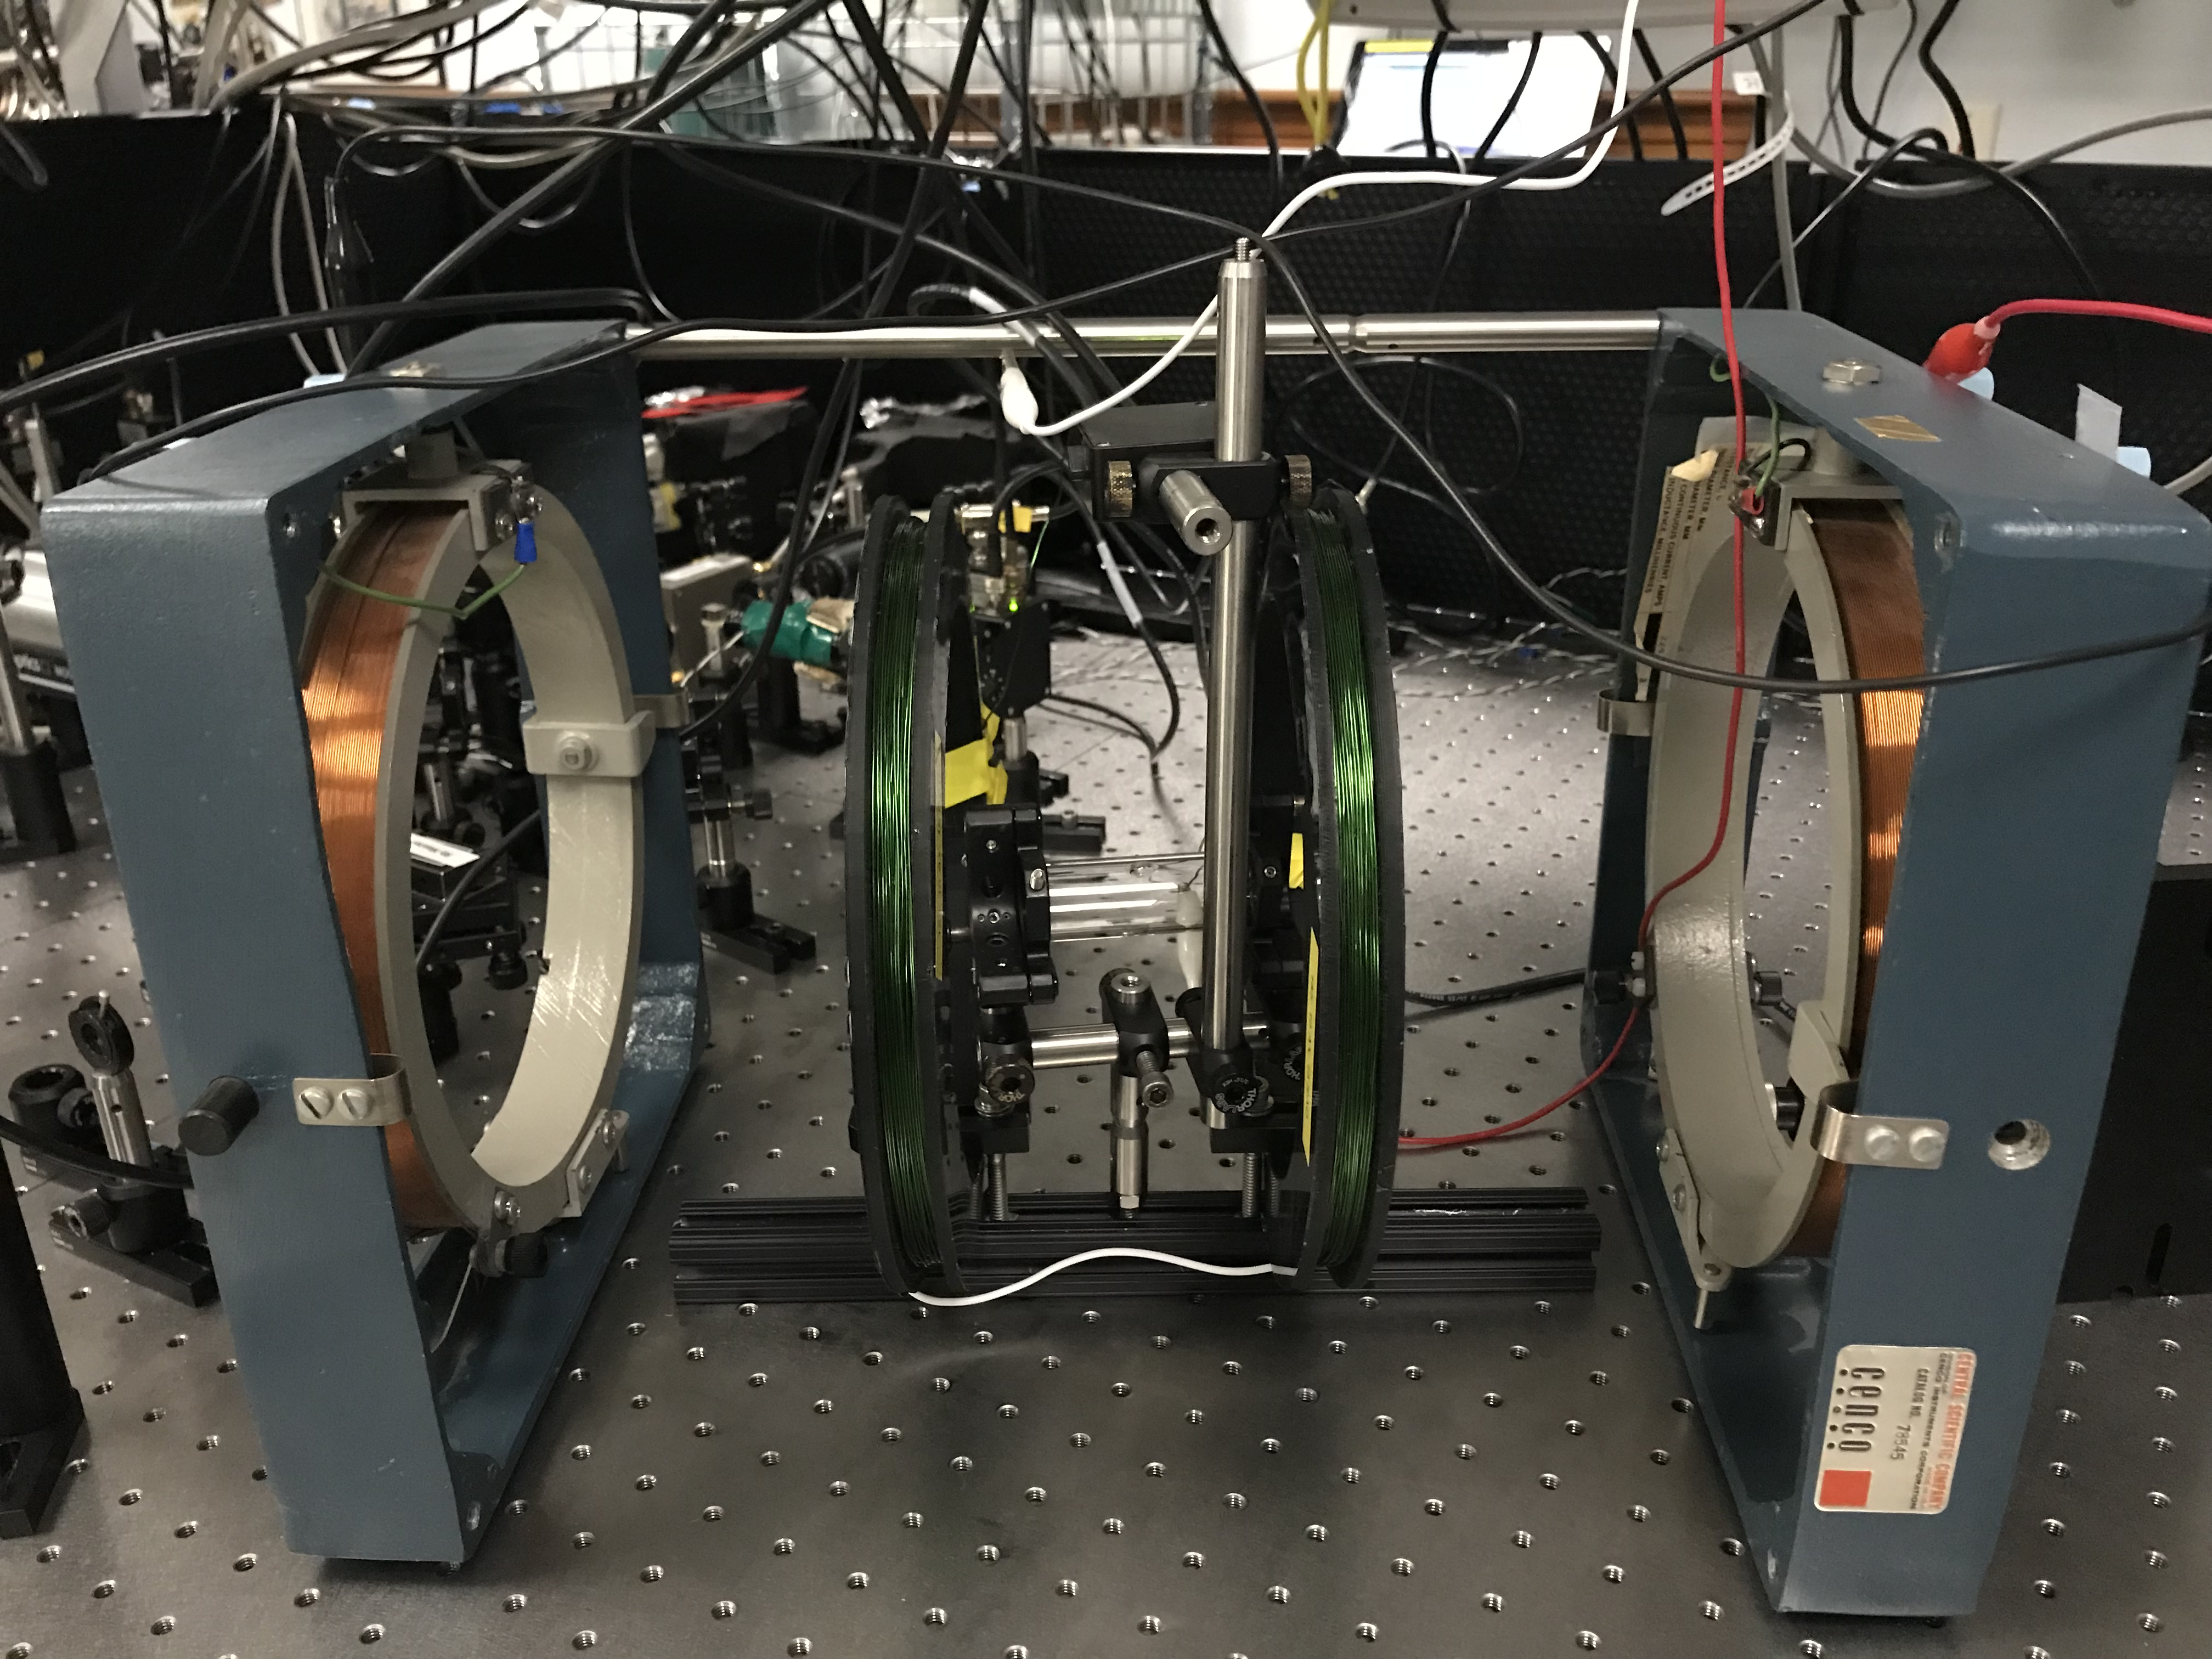
\includegraphics[width=0.8\textwidth]{Images/actualcoils.png}};
	\node[text = white] at (-4,-3.5) {\large Compensation};
	\node[text = white] at (-4,-4) {\large Coils};

	\node[text = white] at (0,-2.7) {\large Main};
	\node[text = white] at (0,-3.2) {\large Coils};

	\draw[red, line width = 1.6pt] (-3.5,-.5) -- (-1.5,-.5);
	\draw[red,->,>=stealth, line width = 1.6pt] (1.65,-.5) -- (3.75,-.5);
	\node[text = white] at (2.5,-1) {\large Laser};
	\node[text = white] at (2.5,-1.5) {\large Beam};

	\node[text = white] at (-1.5,2) {\large Photodiode};
	\end{tikzpicture}
	\caption{Main coils (inside, black) shown along with the compensation coils (outside, blue).}
	\label{fig:actualcoils}
\end{figure}

The expected magnetic field strength along the axial direction and along the radial direction were calculated using computer simulations. These data are shown in Fig. \ref{fig:axialtheoretical}. For a current of \SI{1}{ A}, the expected magnetic field was nearly \SI{13}{ G}, which is more than sufficient for our purposes. Furthermore, the calculation showed a homogeneity of \SI{\pm 0.1}{ Gauss} in the axial direction and of \SI{\pm 0.2}{ Gauss} in the radial direction. These two calculations confirmed that this Helmholtz configuration would supply the necessary magnetic field.

\begin{figure}[htpb]
	\centering
	\begin{minipage}{.49\textwidth}
	\centering
	\begin{tikzpicture}
		\node at (0,0) {\includegraphics[width=0.9\textwidth]{../../Helmholtz/axialtheoretical.pdf}};
		\draw[fill = white,white] (-1,2) rectangle (1,2.5);
		\node[rotate = 90] at (-3.5,0) {\scriptsize Magnetic Field (Gauss)}; 
		\node[] at (0,-2.5) {\scriptsize Axial Distance from Center (m)}; 
	\end{tikzpicture}
	\end{minipage}
	\begin{minipage}{.49\textwidth}
	\centering
	\vspace{.5cm}
	\begin{tikzpicture}
		\node at (0,0) {\includegraphics[width=0.9\textwidth]{../../Helmholtz/radialtheoretical.pdf}};
		\node[rotate = 90] at (-3.5,0) {\scriptsize Magnetic Field (Gauss)}; 
		\node[] at (0,-2.5) {\scriptsize Radial Distance from Center (m)}; 
	\end{tikzpicture}
	\end{minipage}
	\caption{Numerical results for the field strength along the axial and radial direction for our Helmholtz configuration (blue) and a Helmholtz configuration with a longer distance between coils than radius of coils (yellow). The axial and radial dimensions of the rubidium cell are shown in red. Simulation by Dr. Michaela Kleinert.}
	\label{fig:axialtheoretical}
\end{figure}


The support structure was 3D printed in Dr. Daniel Borrero's lab and the wiring was coiled by hand. The strength and homogeneity of the magnetic field were measured with a Gauss meter. The configuration performed as expected, producing a homogeneous magnetic field in both the radial and axial direction. In the axial direction in between the coils, the magnetic field stayed within \SI{\pm 0.25}{ G} for a current of \SI{0.5}{ A} and within \SI{\pm 0.5}{ G} for a current of \SI{1.0}{ A}. A graph of these data is shown in Fig. \ref{fig:FieldAxial} with vertical lines showing the boundary of the coils. In the radial direction for both \SI{0.5}{ A} and \SI{1.0}{ A}, the magnetic field stayed with \SI{\pm 0.25}{ G} for a radius less than \SI{7}{\centi \meter}. Beyond this this radius, the magnetic field decreased significantly. A graph of the radial magnetic field is shown in Fig. \ref{fig:FieldAxial}, with vertical lines showing the boundary of the coils. The rubidium cell, being \SI{8}{\centi \meter} long and having a diameter of \SI{1}{\centi \meter}, is well within the range of homogeneity.


%%%%%%%%%%%%%%%%%%%%%%%%%%%%%%%%%%%%%%%%%%%%%%%%%%
% Axial Magnetic Field
%%%%%%%%%%%%%%%%%%%%%%%%%%%%%%%%%%%%%%%%%%%%%%%%%%
\begin{figure}[h]
		\centering
		\begin{minipage}{.49\textwidth}
			\includegraphics[width = .9\textwidth]{Images/FieldAxial.pdf}
		\end{minipage}
		\begin{minipage}{.49\textwidth}
			\includegraphics[width = .9\textwidth]{Images/FieldRadial.pdf}
		\end{minipage}
		\caption{Graph of the magnetic field along the axial and radial direction for currents of \SI{1.0}{A} and \SI{0.5}{A}.}
		\label{fig:FieldAxial}
\end{figure}


The strength of the magnetic field was measured at the center of the coils as a function of the current through the coils. This allowed a direct calculation of the magnetic field, knowing only the current being supplied to the coils. These data are shown in Fig. \ref{fig:FieldvCurrent} along with a line of best fit. As expected, the relationship between magnetic field strength and current is linear, given by

\begin{equation}
	B = 13.23 I-0.28,
	\label{eq:fieldvcurrent}
\end{equation}
%
where $B$ is the magnetic field in Gauss and $I$ is the current in amperes.

%%%%%%%%%%%%%%%%%%%%%%%%%%%%%%%%%%%%%%%%%%%%%%%%%%
% Field versus current
%%%%%%%%%%%%%%%%%%%%%%%%%%%%%%%%%%%%%%%%%%%%%%%%%%
\begin{figure}[h]
		\centering
		\includegraphics[width = .8\textwidth]{Images/FieldvCurrent.pdf}
		\caption{Graph of the strength of the magnetic field in the center of the Helmholtz coils as a function of current.}
		\label{fig:FieldvCurrent}
\end{figure}

In addition to the coils described above, which we will call the main coils, a second pair of Helmholtz coils was used to compensate for the geomagnetic field and other stray magnetic fields in the lab. These coils, which we will call the compensation coils, were placed outside of the main coils and oriented in the direction of the geomagnetic field. The compensation coils are shown in blue steel housing and copper wiring in Fig. \ref{fig:actualcoils}. They created a homogeneous magnetic field equal and opposite to the geomagnetic field so that the only magnetic field in the experiment was from the main coils.



%%%%%%%%%%%%%%%%%%%%%%%%%%%%%%%%%%%%%%%%%%%%%%%%%%
% Fluorescence Measurements
%%%%%%%%%%%%%%%%%%%%%%%%%%%%%%%%%%%%%%%%%%%%%%%%%%
\chapter{Fluorescence Measurements}
With a laser on resonance with rubidium and capable of being operated in pulsed or continuous wave mode, a magnetic field of variable strength and orientation, and a rubidium cell, the fluorescence of rubidium was measured as a function of the magnetic field strength, magnetic field orientation, repetition rate, and with circularly polarized light compared to linearly polarized light. This chapter describes the final experimental setup, methods for measurements, and the results of these experiments.

\section{Experimental Setup}
The final experimental apparatus is shown as a schematic in Fig. \ref{fig:expsetup} and as a photograph in Fig. \ref{fig:expsetupactual}. It consisted of the diode laser on resonance with the rubidium D$_2$ line and capable of being operated in pulsed or continuous wave mode, the main coils variable in strength and angle with respect to the laser beam, compensation coils to cancel out any stray magnetic fields, the rubidium cell, and two photodiodes to measure fluorescence from the top of the cell (photodiode 1) and to measure backscattered light (photodiode 2). 

\begin{figure}[ht]
	\centering
	\includestandalone[width = .9\textwidth]{Images/tikz/fluorescence}
	\caption{Schematic of the experimental setup to measure fluorescence of rubidium atoms including the Helmholtz coils, rubidium cell, and photodiode.}
	\label{fig:expsetup}
\end{figure}

\begin{figure}[htpb]
	\centering
	\begin{tikzpicture}
		\node at (0,0) {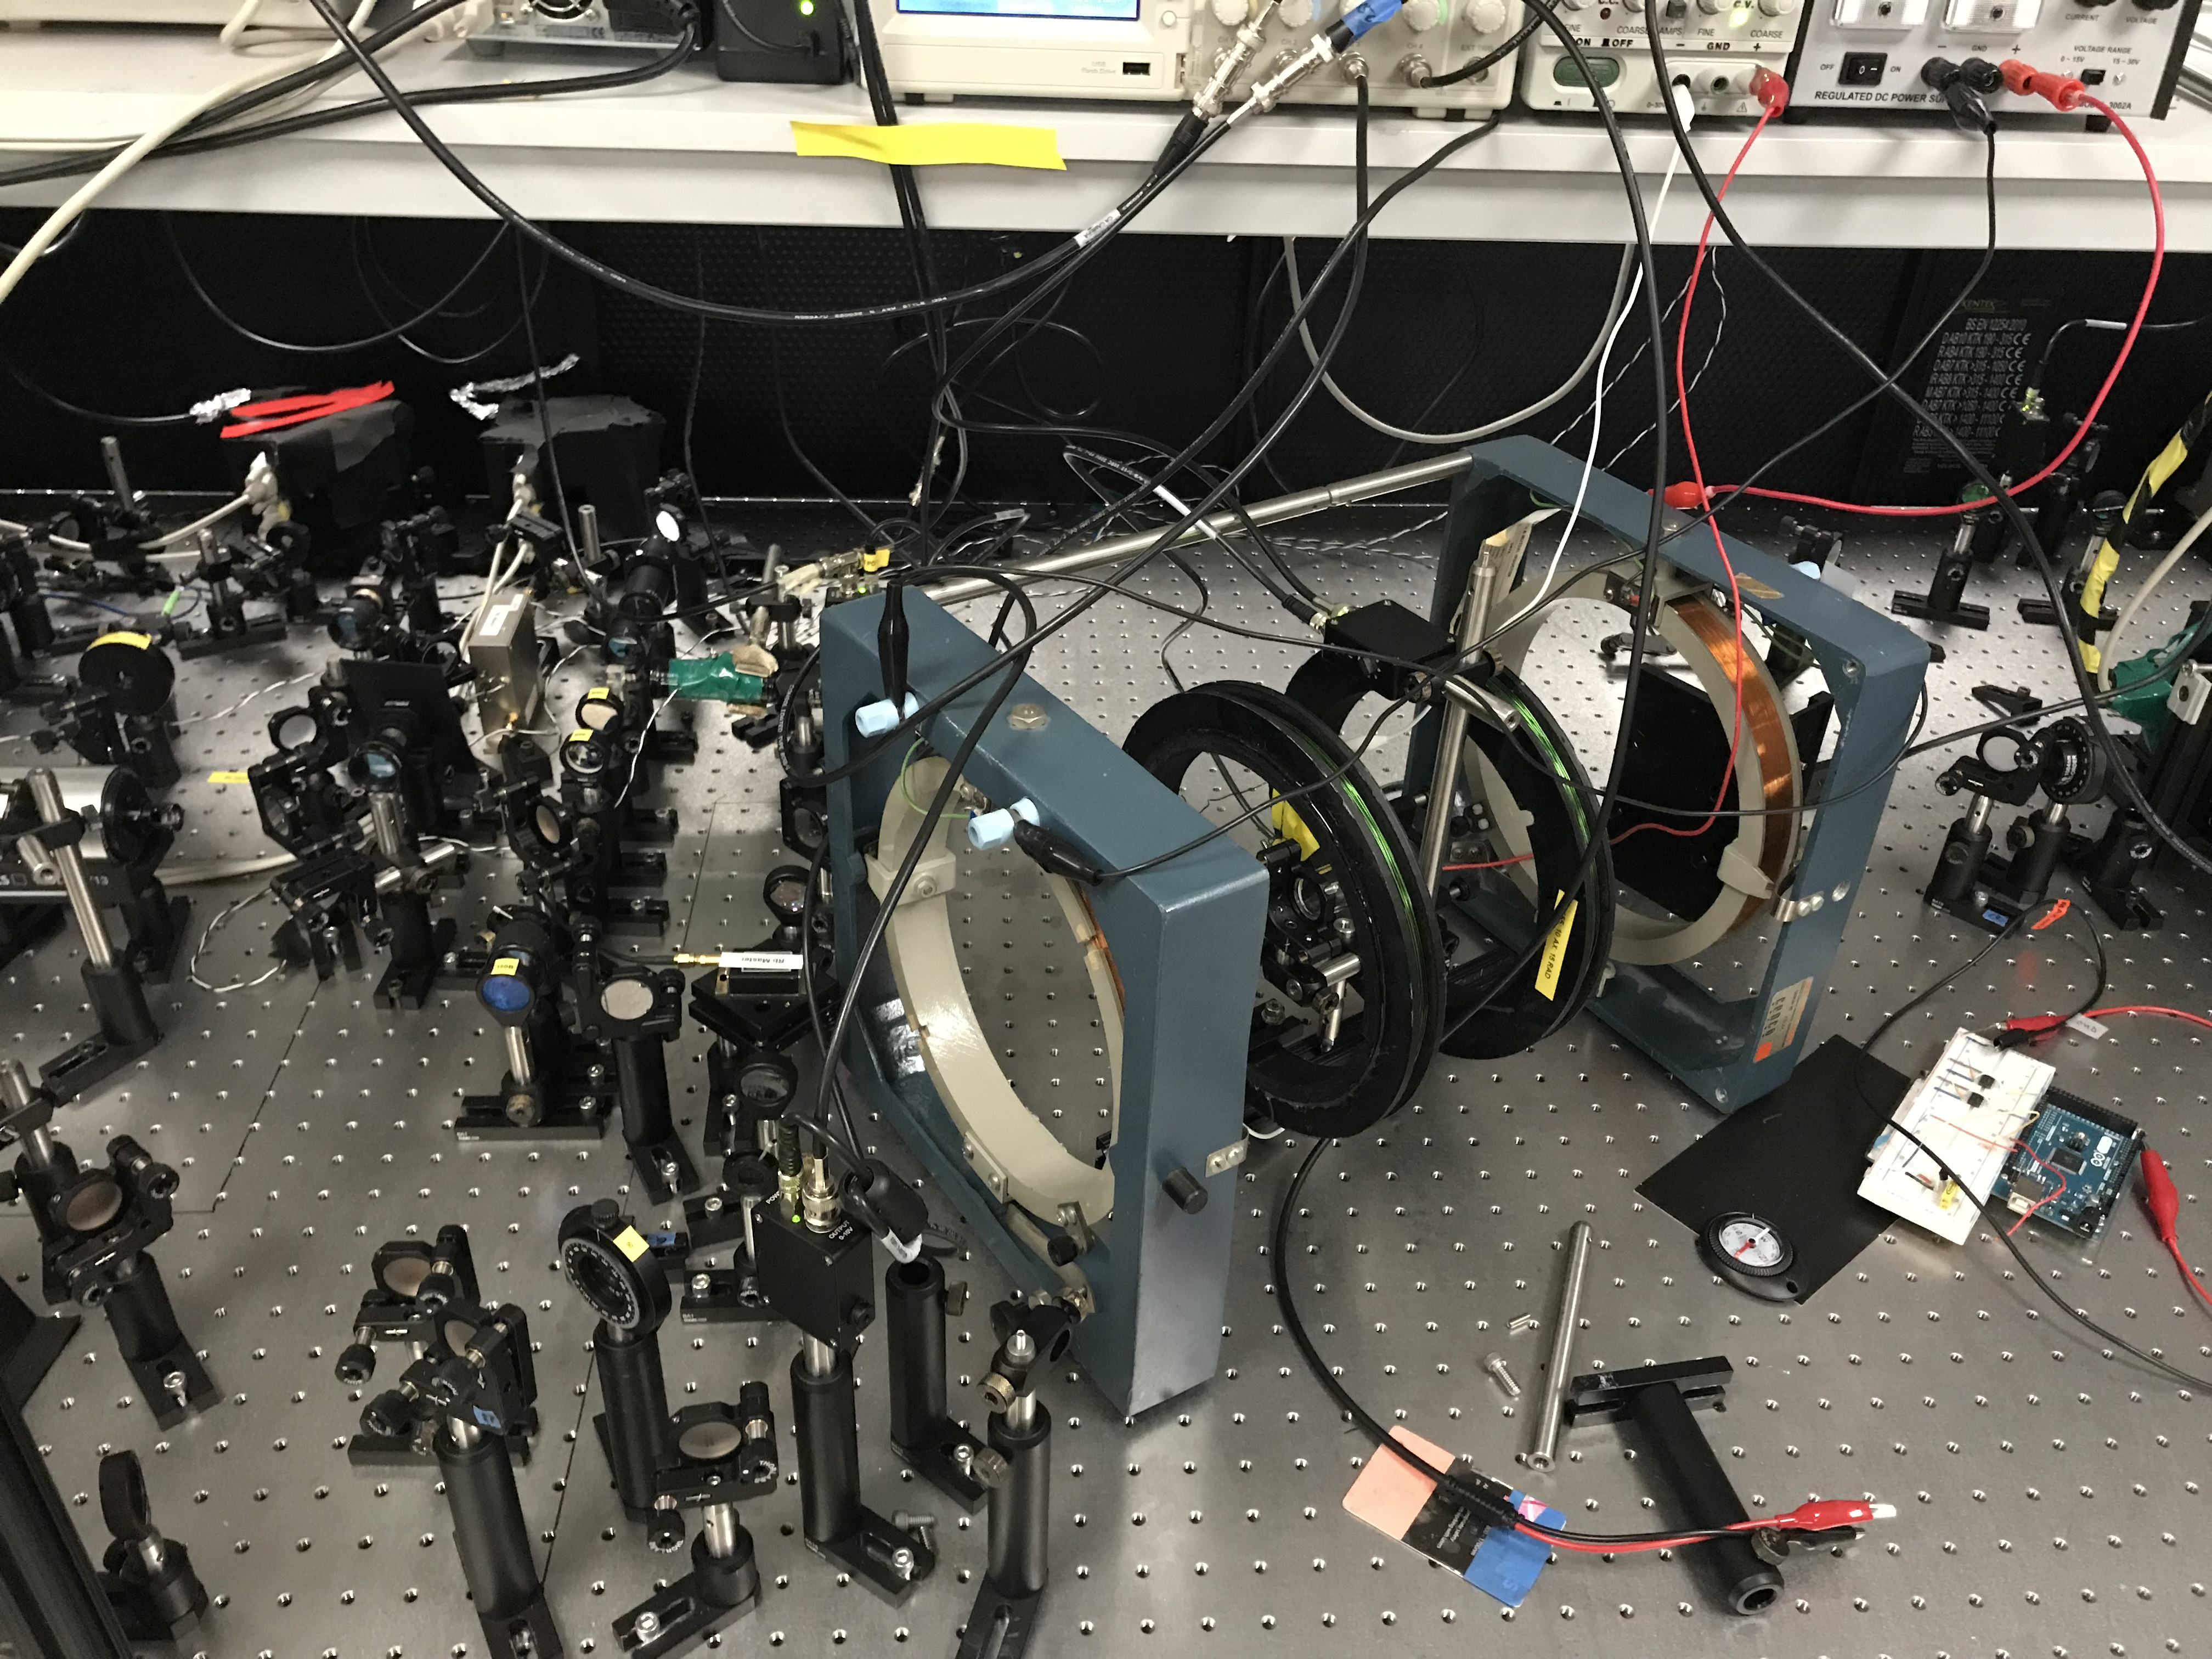
\includegraphics[width=0.8\textwidth]{Images/setup.png}};
		\node[text = white] at (1.5,-3) {\large Compensation};
		\node[text = white] at (.5,-3.5) {\large Coils};
		\node[text = white] at (2,-1.5) {\large Main};
		\node[text = white] at (2,-2.0) {\large Coils};
		\node[text = white] at (0,2) {\large Photodiode};
		\draw[red,->,stealth, line width = 1.6pt] (-2.5,-2.2) -- (-.5,-1.1);
		\node[text = white] at (-3,-1.5) {\large Laser};
	\end{tikzpicture}
	\caption{Experimental setup shown with compensation coils, main coils, absorption cell, and laser beam.}
	\label{fig:expsetupactual}
\end{figure}

The photodiodes were connected to an oscilloscope which was triggered at the scanning frequency of the diode laser. Fluorescence was measured by recording the potential difference from the oscilloscope and dividing it by the average power of the laser. This division is important as it allows us to compare the fluorescence between pulsed and continuous wave laser beams. Without it, the fluorescence from the continuous wave beam would consistently be greater since this beam has a higher average power.

%In order to characterize the fluorescence of rubidium from the constructed laser, a measurement of the saturation intensity of rubidium was taken. This is a measurement of the fluorescence of the atoms as a function of the average power of the laser, and indicates the power at which the atoms are being excited as quickly as possible. Above this intensity, no extra laser power will result in more atoms absorbing and emitting more light. This measurement was made with no magnetic field and the laser operating in continuous wave mode. These data are shown in Fig. \ref{fig:satint}. The error bars come from uncertainty in the fluorescence measurements recorded from the oscilloscope. A best best fit function,
%
%\begin{equation}
%	\text{f} = \frac{1}{1+e^{-1.6 \left( p - 1.1 \right) }},
%	\label{eq:satint}
%\end{equation}
%%
%where f is the fluorescence of the atoms and $p$ is the laser power in milliwatts.
%
%\begin{figure}[htpb]
%	\centering
%	\includegraphics[width=0.8\textwidth]{../../Diode/SatCont.pdf}
%	\caption{Saturation intensity for rubidium pumped with the diode laser operating in continuous wave. A line of best fit is also plotted, given by Eq. \ref{eq:satint}. The error bars come from uncertainty in the fluorescence measurements.}
%	\label{fig:satint}
%\end{figure}



\section{Fluorescence versus Magnetic Field Strength and Repetition Rate}

The first measurement taken was of the fluorescence with respect to the magnetic field strength. With a magnetic field perpendicular to the laser beam and circularly polarized light, we performed this measurement to search for an increase in fluorescence when the repetition rate of the laser matched the Larmor frequency of the atoms. An arbitrary current was chosen (0.12 A) and the magnetic field was calculated using Eq. \ref{eq:fieldvcurrent} (1.3 G). The Larmor frequency of rubidium in this magnetic field was then calculated using Eq. \ref{zeemanf} (610 kHz). The repetition rate of the diode laser was set to this Larmor frequency using the function generator and the current was varied around the 0.12 A, thus changing the strength of the magnetic field. The expected result was an increase in the fluorescence around 0.12 A and this result was found. These data are shown in Fig. \ref{fig:flvc}, with a peak at \SI{0.12}{ A}. The error in the measurements comes from uncertainty in the potential difference read from the oscilloscope (which can be quite large, due to jitter in the laser and electronic noise) and from error in measuring the power of the laser beam. The error was calculated using error porpagation from the uncertainty in each measurement.


\begin{figure}[htpb]
	\centering
	\includegraphics[width=0.8\textwidth]{../../MRPData/EfficiencyCurr.pdf}
	\caption{Fluorescence versus current with magnetic field perpendicular to laser beam and the repetition rate set at \SI{700}{ kHz}. The expected increase at 0.12 A is seen. The error in the measurements comes from uncertainty in the potential difference read from the oscilloscope (which can be quite large, due to jitter in the laser and electronic noise) and from error in measuring the power of the laser beam. The error was calculated using error propagation from the uncertainty in each measurement.}
	\label{fig:flvc}
\end{figure}

The second measurement taken was of fluorescence versus repetition rate with a constant magnetic field perpendicular to the laser beam. With the current set to 0.12 A (a magnetic field of \SI{1.3}{ G}), the expected peak in fluorescence would occur at \SI{700}{ kHz}. The fluorescence indeed peaked at \SI{700}{ kHz}, which can be seen in Fig. \ref{fig:flvrep}. The error comes from uncertainty in the fluorescence measurement as well as uncertainty in the average laser power measurement. Since, for magnetic fields perpendicular to the laser beam, the total angular momentum vector precesses in time about the axis of the field, optical pumping is not as efficient for this orientation as it is when the magnetic field is parallel to the beam. However, this confirmed that MRP can restore the benefits of optical pumping by only ``talking'' to the atoms at one point in their angular momentum's precession. We report a 14\% increase in fluorescence as the repetition rate of the laser is tuned to the Larmor frequency, with a full width at half-maximum of approximately \SI{50}{ kHz}.

\begin{figure}[ht]
	\centering
	\includegraphics[width=0.8\textwidth]{../../MRPData/MAR24/FLvRep.pdf}
	\caption{Fluorescence of rubidium in a magnetic field of approximately 1.3 G perpendicular to laser beam as a function of repetition rate. The peak at \SI{700}{ kHz} shows the increase in fluorescence at the Larmor frequency of the atoms. The error comes from uncertainty in the fluorescence measurement as well as uncertainty in the average laser power measurement.}
	\label{fig:flvrep}
\end{figure}


\section{Fluorescence versus Angle between Laser Beam and Magnetic Field Direction}
We next took measurements of the fluorescence versus the angle between the magnetic field and the laser beam. Measurements were taken with the laser operating in pulsed and continuous wave mode, as well as with linearly and circularly polarized light. The magnetic field was tuned to the repetition rate such that the system was in MRP and there was a maximum in fluorescence. Fluorescence measurements were then recorded at various angles of the magnetic field with respect to the laser beam. A schematic of this is shown in Fig. \ref{fig:flvanglesch}. The results according to Kane et al. \cite{Kane2014} are as follows:

\begin{figure}[htpb]
	\centering
	\includestandalone[width=0.8\textwidth]{Images/tikz/FlvsAngle}
	\caption{Schematic of the rotation of the magnetic field with respect to laser beam.}
	\label{fig:flvanglesch}
\end{figure}


\begin{itemize}
	\item Circularly polarized light operating in pulsed and continuous mode give roughly equal fluorescence at $0^{\circ}$.
	\item As the angle between the magnetic field and laser beam increases, the fluorescence from circularly polarized, pulsed light stays constant while circularly polarized, continuous wave light decreases.
	\item The fluorescence from linearly polarized, continuous wave and linearly polarized, pulsed light should be lower than circularly polarized light, but should stay constant over all angles.
\end{itemize}

The data obtained from our measurements are shown in Fig. \ref{fig:flvangle}. To summarize, our data show the following:
\begin{itemize}
	\item Fluorescence from circularly polarized, pulsed light stays constant over all angles between the magnetic field and the laser beam. Fluorescence from circularly polarized, continuous wave light decreases as the angle increases. This is expected.
	\item The fluorescence from circularly polarized, pulsed light and circularly polarized, continuous wave light is not equal at $0^{\circ}$. Circularly polarized, continuous wave light has the lowest fluorescence overall. This is not expected.
	\item The fluorescence from linearly polarized, pulsed and continuous wave light stays roughly constant over all angles. This is expected.
\end{itemize}

The most important aspect of these data is the different trends seen in the fluorescence from the circularly polarized, continuous wave light and the circularly polarized, pulsed light. For circularly polarized, continuous wave light, the fluorescence should decrease with increasing angle since the magnetic field at increasing angles is redistributing the total angular momenta of the atoms, degrading the benefits of optical pumping. However, with pulsed light, the atoms are only being pumped at one point in their precession cycle. To the light, the atom seems to not be precessing at all, and the benefits of optical pumping are restored. Thus, for all angles, the fluorescence from the circularly polarized, pulsed light should stay constant, which it does.

There are, however, a few concerns with these data. Firstly, the fluorescence from circularly polarized, continuous wave and pulsed light is not equal at $0^{\circ}$. Secondly, circularly polarized, continuous wave light should result in higher fluorescence than linearly polarized, continuous wave light (this is optical pumping, described in Chapter 2), which these data do not show. It is possible that these problems are results of the intensity of the continuous wave light, which was found to be classified in a high intensity regime \cite{Kane2014}. At these intensities, transition saturation (one of the ``three evils'' of LGS, also known as depumping) becomes a  problem. Transition saturation is the decay of atoms to a lower ground state (the second hyperfine ground state) after emission of a photon. Atoms in this lower ground state cannot be excited by our laser since this transition requires a different wavelength for excitation. For high intensities, a significant number of atoms can decay into this lower ground state since atoms are being excited as rapidly as possible. This results in less atoms that can absorb and emit light, thereby decreasing the overall fluorescence (this is described more in the following section). To mitigate the consequences of transition saturation, data were taken with CW light at a lower intensity (a power of around \SI{1}{\milli \watt}). These data, shown in Fig. \ref{fig:flvangle2}, show the correct vertical positions that are expected as well as the same trends seen in the previous data. 


\begin{figure}[htb]
	\centering
	\includegraphics[width=0.8\textwidth]{../../MRPData/MAR24/together.pdf}
	\caption{Fluorescence of rubidium atoms in a magnetic field of approximately 1.3 Gauss as a function of the angle between the field and the laser beam in the high intensity case. Data of pulsed and continuous laser light circularly and linearly polarized are shown. Circularly polarized light with a repetition rate equal to the Larmor frequency gives the highest return for all magnetic field orientations.}
	\label{fig:flvangle}
\end{figure}

\begin{figure}[htb]
	\centering
	\includegraphics[width=0.8\textwidth]{../../MRPData/April16/together.pdf}
	\caption{Fluorescence of rubidium atoms in a magnetic field of approximately a few Gauss as a function of the angle between the field and the laser beam in the low intensity case. Data of pulsed and continuous laser light circularly and linearly polarized are shown. Circularly polarized light with a repetition rate equal to the Larmor frequency gives the highest return for all magnetic field orientations.}
	\label{fig:flvangle2}
\end{figure}

In order to look at overall trends and to better visualize the changes in fluorescence with increasing angle, we calculate the percent of maximum fluorescence, and plot them as well in Fig. \ref{fig:flvanglescaled}. We report a 33\% decrease in fluorescence for continuous wave, circularly polarized laser beams and a 2\% decrease in fluorescence for MRP laser beams at an angle of $90 ^{\circ}$ between the laser beam and the magnetic field.

\begin{figure}[htb]
	\centering
	\begin{minipage}{.48\textwidth}
	\centering
		\includegraphics[width=0.9\textwidth]{../../MRPData/April16/togetherscaled.pdf}
	\end{minipage}
	\begin{minipage}{.48\textwidth}
	\centering
		\includegraphics[width=0.9\textwidth]{../../MRPData/MAR24/togetherscaled.pdf}
	\end{minipage}
	\caption{Percent of maximum fluorescence with respect to the maximum of rubidium atoms in a magnetic field of approximately 1.3 G as a function of the angle between the field and the laser beam. The low intensity case is shown on the left and the high intensity case shown on the right. Data of pulsed and continuous laser light circularly and linearly polarized are shown. Circularly polarized light with a repetition rate equal to the Larmor frequency gives the highest return for all magnetic field orientations.}
	\label{fig:flvanglescaled}
\end{figure}

\subsection{Repumping}
The transition we have been looking at so far is the $D_{2}$ transition, which is an excitation from the F = 2 to the excited state. As mentioned earlier and described in other papers \cite{Kane2014}, it is possible for atoms to decay into the lower ground state, F = 1, which cannot be accessed by our laser. This results in atoms falling into a dark state, causing an overall decrease in fluorescence. Thus, we introduced a repumper laser capable of accessing this transition. This would allow atoms in the second hyperfine ground state to be excited, thereby allowing that atom to contribute to the overall fluorescence. We theorized that the addition of this repumper would correct the incorrect vertical scale for circularly polarized, continuous wave light, seen in Fig \ref{fig:flvangle}. 

The repumper consisted of the same diode laser as described Section 3.2. However, the diffraction grating for this laser has a slightly different angle than the main laser, thus changing its wavelength enough to access the excitation from the second hyperfine ground state. The repumper beam was overlapped with the main laser beam using a polarizing beam splitting cube. This resulted in the repumper beam having linear polarization orthogonal to the main laser beam polarization. This results in the repumper beam having $\sigma^{-}$ circular polarization after linear to circular polarization conversion. As mentioned earlier, the main laser has $\sigma^{+}$ circular polarization.

We measured the fluorescence at $0^{\circ}$ and at $90^{\circ}$ between the laser and magnetic field for varying levels of repumper laser power. The fluorescence measurements were taken with three different levels of repumper percentages (rempumper power divided by main laser power): 0\%, 10\%, and 20\%. The data of these three levels are shown in Fig. \ref{fig:0repump}. We did not find the addition of the repumper to increase fluorescence for the pulsed laser. Instead, we found the opposite to be true! As repumper percentage increases, the fluorescence from the pulsed laser \textit{decreases} significantly.

\begin{figure}[htpb]
	\centering
	\includegraphics[width=0.9\textwidth]{../../MRPData/Repumping/20scaled.pdf}
	\caption{Fluorescence as percentage of maximum fluorescence versus the angle between the laser beam and magnetic field is shown for repumper percentages of 0\%, 10\%, and 20\%. The dashed lines do not constitute data but are shown to guide the eye.}
	\label{fig:0repump}
\end{figure}


We believe this trend to be true because of the polarization and CW mode of the repumper. The repumper has $\sigma^{-}$ circular polarization, which pushes atoms into lower angular momentum states as opposed to the main laser, which pushed atoms into higher angular momentum states. We can quickly and \textit{roughly} estimate if this is significant or not. The main laser has a repetition rate of \SI{700}{\kilo Hz} and a duty cycle of 20\%. Thus, each pulse width is about \SI{0.28}{\micro \second}. In this time, a cycling transition needs to be established. Since the  repumper is on all the time (continuous wave), it has a very large amount of time (compared to the main pulsed laser) to push atoms into the lowest angular momentum state, $m_F = -4$. Then as the main laser pumps the atoms, it will take roughly 10 transitions to get to the cycling transition of highest angular momentum (there are only 7 transitions, but each transition has roughly a 1/3 probability\footnote{The probability is actually not 1/3, nor do the transitions have the same probability. We use a 1/3 probability in order to get a rough estimate. See Steck (2001) for more information on decay rates \cite{steck}.} of decaying into a lower angular momentum state). The life time of an excited state is \SI{1.6e-8}{\second} \cite{steck}. Thus, it will take \SI{0.26}{\micro \second} to reach a cycling transition. However, this is roughly the pulse width, so in the time that it takes the atoms to get into the cycling transition, the pulse has ended and the repumper pushes the atoms back down to the lowest angular momentum state, undoing the whole effort. Thus, the cycling transition cannot be maintained. Going forward, the repumper should be pulsed along with the main laser so that it is only acting in conjunction with the main laser. Furthermore, the repumper should have the same polarization as the main laser so that it does not push atoms down to lower angular momentum states but instead pushes atoms towards higher angular momentum states where a cycling transition can be established.

Lastly, we wanted to fix some of the problems we found with the first fluorescence versus angle data taken, shown in Fig. \ref{fig:flvangle}. It was seen that the fluorescence from the circularly polarized, continuous wave light was significantly lower than the fluorescence from the circularly polarized, pulsed light, which was not expected. We thought that this might be due to the transition saturation, and theorized that a repumper would fix this problem. We thus retook this data for circularly polarized, pulsed light at \SI{1.5}{\milli W}, circular continuous light at \SI{6}{\milli \watt} without a repumper, and circular continuous light at \SI{6}{\milli W} with 20\% repumper. These data are shown in Fig. \ref{fig:flvanglerepump}, and it is seen that the repumper indeed increases fluorescence to the proper vertical position. This confirmed that transition saturation was occurring for laser beams with high intensity in our data.

\begin{figure}[htpb]
	\centering
	\includegraphics[width=0.8\textwidth]{../../MRPData/Repumping/transat.pdf}
	\caption{Fluorescence versus angle for circular pulsed light, circular continuous light, and circular continuous light with the repumper.}
	\label{fig:flvanglerepump}
\end{figure}

\subsection{Backscatter Fluorescence}
All of the previous data were measured using photodiode 1 (from top down) since this allowed the collection of light to not be interrupted with the rotation of the main coils. In order to ensure that backscatter fluorescence indeed followed these same trends (since telescopes rely on the backscattered light from laser guide stars), we took two data points, at $0^{\circ}$ and $90^{\circ}$ measured with photodiode 2 (backscatter). Only two data points were taken because, for many angles, the main coils were in between the rubidium cell and the photodiode. These data confirm that MRP behaves similarly when measuring backscatter. These data are shown in Fig. \ref{fig:backscatter} as the raw data and as percentage changes from maximum fluorescence. The backscatter fluorescence was shown to decrease by nearly 18\% for a change in angle from $0^{\circ}$ to $90^{\circ}$.

\begin{figure}[htb]
	\centering
	\begin{minipage}{.49\textwidth}
	\centering
		\includegraphics[width=0.9\textwidth]{../../MRPData/Backscatter/backscatter.pdf}
	\end{minipage}
	\begin{minipage}{.49\textwidth}
	\centering
		\includegraphics[width=0.9\textwidth]{../../MRPData/Backscatter/backscatterScaled.pdf}
	\end{minipage}
	\caption{Fluorescence for circularly polarized light with continuous light and pulsed light at the Larmor frequency; raw data is shown on the left and percent changes from maximum fluorescence data on the right. It is seen that backscatter agrees well with the data taken from top down. The dashed lines do not constitute data but are shown to guide the eye.}
	\label{fig:backscatter}
\end{figure}




%%%%%%%%%%%%%%%%%%%%%%%%%%%%%%%%%%%%%%%%%%%%%%%%%%
% Conclusion
%%%%%%%%%%%%%%%%%%%%%%%%%%%%%%%%%%%%%%%%%%%%%%%%%%
\chapter{Conclusion}
In this thesis, we introduce laser guide stars and describe an inherent problem that hampers their efficiency: Larmor precession. We thoroughly explain the theory behind laser guides stars and the theory behind the problem of Larmor precession that degrades the brightness of laser guide stars. From this, we identify a possible solution to increase the brightness of laser guide stars: magnetic resonant pulsing. The theory of magnetic resonant pulsing is explained and an experiment to test magnetic resonant pulsing is presented and demonstrated.

We confirm that magnetic resonant pulsing indeed results in an increase in fluorescence. For circularly polarized light and a pulsed laser beam, we report a 14\% increase in fluorescence between repetition rates that are out of and in resonance with the Larmor precession. Furthermore, we show that for circularly polarized light, magnetic resonant pulsed light decreases in fluorescence by only 2\% when the angle between the magnetic field and laser beam increases from $0^{\circ}$ to $90^{\circ}$. In contrast, a continuous wave laser decreases by 32\% when the angle between the laser beam and magnetic field increases from $0^{\circ}$ to $90^{\circ}$.

These data show that laser guide star systems at most latitudes would benefit from magnetic resonant pulsed lasers. A significant challenge with this, however, would be matching the repetition rate of the laser to the Larmor frequency of the atom. The precise value of the geomagnetic field is not always known, and thus a laser system capable of variable repetition rate would be needed in order to lock to magnetic resonant pulsing. 

However, there is still much more work that can be done in this area. One significant problem encountered in this experiment was measuring the fluorescence while changing the magnetic field strength, orientation of the magnetic field, or the repetition rate. One of these parameters would be changed, and a measurement would be recorded manually from the oscilloscope. This took around \SI{30}{\second} per measurement and for approximately 20 measurements, this time would add up. In this time, it was possible for the diode laser to stray off resonance, affecting the fluorescence measurements significantly. For future experiments, this should be taken into consideration. Possible solutions would be a more stable laser source or a computerized system to instantly record values from the photodiode. We considered an Arduino system that would read analog voltages at sub-millisecond intervals to a computer, but did not have time to implement this.

Another problem was generating a precise magnetic field and compensating for the geomagnetic field. For studies looking at this effect with greater precision, it would be beneficial to use a magnetic field shield in order to rid the system of all stray magnetic fields. A shield using MuMetal was considered but turned out to be too costly. This would allow for greater accuracy in the angle between the magnetic field and laser beam. This could also be done using a system of three Helmholtz coils along the three Cartesian axes.

An area that should be explored in more detail is that of the duty cycle of the laser. Our laser had a minimum duty cycle of 20\%. This meant that laser light was interacting with the atoms for 20\% of their Larmor precession. In this time, a significant change in the atoms' total atomic angular momentum vector is occurring, decreasing the benefits of optical pumping. A duty cycle of 20\% is found numerically to be optimal \cite{Rampy2010}, but lower duty cycles could result in further increases the benefits of magnetic resonant pulsing, and should be studied further.

Furthermore, the transition saturation problem should also be further investigated as this is not completely independent from Larmor precession. Transition saturation occurs when a significant number of atoms transition into the lower ground state (F=1) of rubidium, becoming inaccessible to excitation from laser light. Adding the repumper at different intensities will shed more light onto this problem. In addition, the polarization and repetition rate of the repumper could be varied.

Another area to look at is the fluorescence versus power of the laser while in magnetic resonant pulsing. Performance of laser guide stars with respect to power have been studied \cite{Holzlohner2012}, but not in magnetic resonant pulsed systems, and it would be beneficial to study this area and look into saturation intensities. The spot size of the laser guide star is another area that has been studied, \cite{Holzlohner2012} and could be studied in this system by varying the width of the laser beam.


%%%%%%%%%%%%%%%%%%%%%%%%%%%%%%%%%%%%%%%%%%%%%%%%%%
% Appendix
%%%%%%%%%%%%%%%%%%%%%%%%%%%%%%%%%%%%%%%%%%%%%%%%%%
%%%%%%%%%%%%%%%%%%%%%%%%%%%%%%%%%%%%%%%%%%%%%%%%%%
% Adam Newton Wright
% Appendix: LGS and Adaptive optics
% app.tex
%%%%%%%%%%%%%%%%%%%%%%%%%%%%%%%%%%%%%%%%%%%%%%%%%%

\appendix

%%%%%%%%%%%%%%%%%%%%%%%%%%%%%%%%%%%%%%%%%%%%%%%%%%
% Laser Guide Stars
%%%%%%%%%%%%%%%%%%%%%%%%%%%%%%%%%%%%%%%%%%%%%%%%%%
\chapter{Laser Guide Stars}

Telescopes observing distant astronomical objects face a significant challenge known as atmospheric distortion. Light coming from these astronomical objects travels in a straight line with little obstruction in the near vacuum of space. However, as a ray of light travels from free space into the atmosphere of Earth, it is affected by the many gaseous particles that make up the atmosphere and result in a different index of refraction than space. The effect is a bending of the light rays, known as \textit{refraction}, that can be described mathematically by Snell's Law, 

\begin{equation}
  n_1 \sin \theta_1 = n_2 \sin \theta_2,
  \label{snellslaw}
\end{equation}
%
where $n_1$ is the index of refraction of the first medium, $n_2$ is the refractive index of the second medium, and $\theta_1$ and $\theta_2$ are the angles that the ray makes with the normal to the interface between the media. A schematic of this is shown in Figure \ref{snellsfigure}.

\begin{figure}[ht!]
  \center
  \includestandalone{Images/tikz/snells}
\caption{Schematic of a ray of light refracting according to Snell's Law as it passes from a medium of refractive index $n_1$ into a medium with higher refractive index $n_2$.}
\label{snellsfigure}
\end{figure}

In general, the many light rays that make up the observed object will be refracted uniformly, causing the object to be perceived in a location that is different from its true position. While that alone is not a problem, if we look closer, we find that the atmosphere does not refract all light rays in the same manner, but small variations in pressure, temperature, and density cause a spatial variation in the index of refraction, resulting in light rays that are close together to be refracted in slightly different ways. This is known as \textit{atmospheric distortion}. A schematic is shown in Figure \ref{fig:atmosphericdistortion}, with plane waves being distorted as they pass through an atmosphere.


\begin{figure}[ht]
  \centering
  \includestandalone{Images/tikz/atmdistortion}
  \caption{Atmospheric distortion of a plane wave passing through Earth's atmosphere}
  \label{fig:atmosphericdistortion}
\end{figure}

The idea of atmospheric distortion will be familiar to those who have seen the sunset on the horizon. As the sun nears the horizon, the light is bent strongly through the atmosphere, resulting in much more distortion than when high in the sky. This results in a disfiguring of its spherical shape and a sharpening around the edges. An example of this is shown in Figure \ref{fig:sunset}.

\begin{figure}[t]
  \centering
  \includegraphics[width = .8\textwidth]{Images/sunset.jpg}
  \caption{Sunset with atmospheric distortion disfiguring the spherical shape of the sun and creating sharp patterns on the edges \protect\cite{sunset}.}
  \label{fig:sunset}
\end{figure}

In order for telescopes to improve resolution, astronomers need to find a way to rid their systems of this atmospheric distortion. One way to do this is to place the telescope outside of Earth's atmosphere where it would be unaffected by atmospheric distortion. This was done with amazing success in 1990 with the low-orbiting, powerful Hubble telescope \cite{Okolski}. However, it is not only extremely costly to put telescopes into orbit, but also impractical as they cannot be easily maintained or serviced.


Thus, a different solution was proposed. If astronomers could model how light was distorted as it passed through the atmosphere, they could subtract those distortions from their images and obtain higher resolution data. In order to measure the amount of distortion present, telescopes can observe a point source in the sky, such as a distant star, and observe its image. This image is then compared with the image of an ideal point source not affected by atmospheric distortion, and the difference between these two images represents the amount of distortion. Once the distortion is known, it is sent to a deformable mirror, which is made of many smaller mirrors, each able to move independently from the others. The deformable mirror can then create a wavefront conjugate to the distortion calculated. By reflecting the image of astronomical object off this mirror, the distortion is removed from the image. This process is known as \textit{adaptive optics}, and more information is given in Appendix B.


However, there are not always stars bright enough in the telescope's field of view that can be used as this point source (better known as a guide star) \cite{Wizinowich2006}. In order to skirt this problem, artificial stars were constructed, known as \textit{laser guide stars} (LGS). A laser guide star is created by sending laser light into the atmosphere, where it interacts with a layer of sodium atoms. These sodium atoms reside approximately $\SI{60}{\kilo\meter}$ from Earth in a $\SI{10}{\kilo\meter}$ thick layer of the atmosphere known as the mesosphere. A figure of this region within the layers of Earth's atmosphere is shown in Figure \ref{fig:mesosphere}. These atoms are deposited from meteors as they burn up in Earth's atmosphere, leaving behind their composite particles, a significant portion being sodium. The density of this sodium layer varies throughout a given day and throughout the year, but typically is near $\SI{5e13}{atoms \per \meter \cubed}$ \cite{Kibblewhite2009}. Using a laser with a wavelength resonant with sodium,  the atoms will absorb and emit this light, creating a glowing sphere in the upper atmosphere, as mentioned in Chapter 2. This sphere of light is then used as the guide star.\footnote{There are actually two types of laser guide stars: sodium based and Rayleigh scattering based. Rayleigh scattering laser guide stars rely on the scattering of light in the atmosphere, as opposed to having atoms absorb and emit light.}

\begin{figure}
		\center
		\includestandalone{Images/tikz/mesosphere}
	\caption{Schematic of sodium atoms residing in the mesosphere.}
	\label{fig:mesosphere}
\end{figure}



In general, most large-scale, ground-based telescopes now have powerful lasers with wavelengths precisely tuned to be resonant with sodium. As these telescopes are making observations, the lasers are shone into the sky to create the LGS. An image of an LGS being created is shown in Figure \ref{fig:LGSatESO}. The LGS is observed and atmospheric distortions are calculated and subtracted from the image in real time.

\begin{figure}[hb!]
  \centering
  \includegraphics[width = .8\textwidth]{Images/LGSatESO.jpg}
  \caption{Laser guide star being created at the Very Large Telescope \protect\cite{VLT}.}
  \label{fig:LGSatESO}
\end{figure}

One major concern for LGS systems is their brightness in the sky \cite{Wizinowich2006}. It is important for the star to be bright enough that the telescope system is able to pick up enough light for a measurement of the distortion. The shape of the LGS is also important, as it must be as near to circular as possible in order for an accurate measurement of the distortion to be made. The shape of the LGS is mostly due to the profile of the laser beam \cite{Holzlohner2012} and will not be discussed here.

In order to create a brighter laser guide star, a few methods are utilized. One method is to increase the intensity, the power per unit area, of the laser. Typical laser intensities are of the order of \SI{20}{W \per \meter \squared} \cite{Kane2014}. This allows for more atoms to absorb and emit light, thereby creating a brighter star. Another method is to increase the diameter of the laser beam, which will allow for a greater area of sodium atoms to be reached by the light. These both have limitations, however. The power cannot continually be increased because of limitations on the power of lasers and due to downpumping \cite{Kane2014}. The size of the LGS also should not be continually increased since, for adaptive optics to work, the assumption is made that the LGS is a point source. A more sophisticated method, optical pumping (discussed in Chapter 2), makes use of circularly polarized light to move the atom into a cycling transition. The method explored in this thesis expounds on using circularly polarized light, but realizes the effects of the geomagnetic field on the distribution of angular momentum when circularly polarized light is used, and uses a pulsed laser to counteract this.


%%%%%%%%%%%%%%%%%%%%%%%%%%%%%%%%%%%%%%%%%%%%%%%%%%
% Adaptive Optics
%%%%%%%%%%%%%%%%%%%%%%%%%%%%%%%%%%%%%%%%%%%%%%%%%%

\chapter{Adaptive Optics}
The process of measuring the atmospheric distortion in order to enhance astronomical imaging, known as \textit{adaptive optics}, is a mathematical estimation problem. Here, we present an introduction to the methods used during this process.

In general, telescopes observe the LGS and the astronomical object simultaneously. The image of the LGS is then compared to an ideal point source imaged through the telescope without atmospheric distortion,\footnote{This is typically done using optical modelling software, but can also be done experimentally using various quasi-pointlike source objects.} and the distortion is calculated by comparing the two. A deformable mirror, composed of many smaller mirrors each of which can be moved independently of the others, is then used to create the opposite of the calculated distortion. The image of the astronomical object is then reflected off this mirror, thereby ridding the image of distortion.

In order to calculate the atmospheric distortion, astronomers make use of the well defined way in which point sources are imaged through optical systems. When an idealized point in object space is imaged through an optical system, it has a certain intensity distribution in image space, known as the point spread function. For an optical system with spherical symmetry and no aberration, the point spread function can be described mathematically along the radial coordinate $x$ as

\begin{equation}
	P(x) = \left(\frac{2 J_1(x)}{x}\right) ^{2},
  \label{psfa}
\end{equation}
%
where $P(x)$ is the intensity and $J_1(x)$ is the Bessel function of the first kind. This function is known as the \textit{Airy disk}, and is shown in Figure \ref{fig:airydiska}. It is an idealized description of a point imaged through a perfect optical system.

%\begin{figure}[h]
%  \centering
%  \begin{tikzpicture}
%	\begin{axis}
%	  \addplot3[surf,z buffer=sort,domain=-5:5,y domain=-5:5] gnuplot {airy((x**2+y**2)**(1/2))};
%	\end{axis}
%\end{tikzpicture}
%  \caption{<+caption text+>}
%  \label{fig:<+label+>}
%\end{figure}<++>




\begin{figure}[h]
  \centering
  \includegraphics[scale = .4]{Images/airydisk.png}
  \caption{Graph of the Airy disk function where the height represents the intensity and the $x$ and $y$ axes represent spatial coordinates. The Airy disk describes an idealized point imaged through a spherically symmetric, aberration free optical system.}
  \label{fig:airydiska}
\end{figure}

It turns out that stars are very close to being point sources and can thus be used as this idealized point source. Since the light from these stars is passing through Earth's atmosphere, it will be distorted, and these distortions will show up in the point spread function, thus deviating from the Airy Disk described by Equation \ref{psfa}. 

Astronomers then use a combination of Fourier mathematics and an optimization algorithm to calculate the distortion. This method follows that outlined by Gonsalves \cite{Gonsalves1982}. This is done by first calculating optical transfer function

\begin{equation}
  H(\omega) = A(\omega) e^{i \theta(\omega)},
  \label{opticaltransfera}
\end{equation}
%
where $A(\omega)$ is the Fourier transform of the aperture function\footnote{The aperture function is a function describing where light can and cannot pass through. For a circular aperture, it would consist of a solid circle where light can pass through and nothing around the circle. It essentially acts like the computational version of a camera aperture.} of the system and $\theta(\omega)$ is the phase of the incoming light. The phase of the light can be described as a summation,

\begin{equation}
  \theta (\omega) = \sum _{k=0} ^{\infty} c_k \phi (\omega),
  \label{phasesuma}
\end{equation}
%
where $\{\phi (\omega) \}$ is a set of polynomials\footnote{The idea of using a set of polynomials to described the phase is similar to the idea of using sinusoidal functions in Fourier analysis to deconstruct a signal.} and $c_k$ is a coefficient that quantifies how much of each polynomial is present in the distortion. Taking the inverse Fourier transform and then the modulus squared, we can calculate the point spread function of this light

\begin{equation}
		P(x) = \Big|\text{ifft}[H(\omega)]\Big|^2,
  \label{otftopsfa}
\end{equation}
%
where $\text{ifft}$ denotes the inverse Fourier transform of the argument. This method allows us to mathematically create a point spread function simply by estimating the phase of the light with a set of polynomials.

Using this method, we have a way to estimate the distortion present in an image. First, a set of polynomials is selected. A possible set of polynomials to use is the Zernike set \cite{Gonsalves1982},\footnote{The Zernike set of polynomials can be used to described many optical distortions such as spherical aberration, defocus, coma, etc., and is chosen for systems displaying these distortions} but there are many others that can be used. Second, a coefficient list, or ``vector,'' of numbers is created in which each number will be the coefficient in front of its corresponding polynomial in the set of polynomials. This gives us a way to weight each of the polynomials in the set. Next, an algorithm is set up to change each number in the coefficient list, and, at each change, the point spread function is calculated (by the method above). This calculated, or estimated, point spread function is then compared to the observed point spread function, and an error metric is calculated. The algorithm will seek to minimize this error metric. Once this is minimized, the calculated point spread will be quite similar to the observed point spread function, and, at this point, we know the distortion acting on the system. The distortion is simply the set of polynomials, each weighted by its coefficient found by the algorithm.


Searching for the correct polynomials weighted by the correct coefficients is not trivial. Sometimes certain polynomials can be ignored if it is known by symmetry that they will not show up in the point spread function. Regardless, searching for the correct distortion is an optimization of a function in a large parameter space. Typical algorithms use a steepest descent approach \cite{Gonsalves1982}, which changes one parameter at a time, calculates an error between that estimation and the observed point spread function, and seeks to minimize this error. There have also been algorithms that use random searches, Monte Carlo walks, and Markov chain Monte Carlo searches that claim robustness and speed \cite{fienup}.

Once the correct distortion is calculated, the information is sent to the deformable mirror. This mirror consists of many smaller mirrors, each of which can be precisely adjusted by a piezoelectric actuator. The mirror changes shape, or adapts to the distortion,\footnote{This is where the term ``adaptive optics'' comes from.} creating a conjugate wavefront that the image from the telescope can be reflected off. At this point, the atmospheric distortion has been removed from the image. Normally, this is done in real time, and thus speed of both the calculation algorithm and of the movement of the deformable mirror must be optimized. Systems typically can calculate and adjust in under a second \cite{Wizinowich2006}.


%\begin{equation}
%  \begin{split}
%	Z_n^m (\rho,\phi) &= R_n^m (\rho) \cos(m\phi)\\
%	Z_n^{-m} (\rho, \phi) & = R_n^m (\rho) \sin(m\phi)\\
%	R_n^m (\rho) & = \sum _{k=0} ^{\frac{n-m}{2}} \frac{(-1)^k (n-k)!}{k!(\frac{n+m}{2}-k)! (\frac{n-m}{2}+k)}
%  \end{split}
%  \label{zernike}
%\end{equation}


%%%%%%%%%%%%%%%%%%%%%%%%%%%%%%%%%%%%%%%%%%%%%%%%%%
% Dye Lasers
%%%%%%%%%%%%%%%%%%%%%%%%%%%%%%%%%%%%%%%%%%%%%%%%%%

\chapter{Dye Lasers}
Dye lasers were some of the first lasers to be used as laser guide stars \cite{Primmerman1991}. This is due to a variety of factors: their wavelength can be precisely tuned over a broad spectral range, they are relatively inexpensive and easy to use,\footnote{Debatable once dye solution has spewed across half of the laboratory floor or fountained over the vacuum chamber. Also, some dyes cost 10 times more than gold per gram, likely invoking bitter feelings when one has to wipe up spilled liquid ``gold.'' Shout out to the LDS-798 backed currency though!} and they are fairly robust. However, recently many telescopes have opted for solid state or fiber lasers because of their efficiency and reliability \cite{Wizinowich2006}. My previous research dealt extensively with dye lasers, which is the main reason an MRP dye laser was first experimented with. Although it ultimately did not function as needed, we describe dye lasers in general, our proposed setup, and the problems that we encountered in this chapter.

\section{Introduction to Dye Lasers}
Laser is an acronym for \textit{light amplification by stimulated emission of radiation}. In general, a laser consists of three parts: a pump, a medium, and a cavity. The pump provides enough energy to move atoms in the medium into an excited state. The atoms then decay back into their ground state, releasing a photon in a random direction, which is known as spontaneous emission. However, a spontaneously emitted photon travelling through the medium can interact with another excited atom and stimulate the emission of a second photon through a process known as stimulated emission. This causes the excited atom to decay to its ground state, releasing a photon with the same direction, frequency, phase, and polarization as the initial photon. A cavity can be created around the medium, typically by placing mirrors on either side of the medium, causing the photons to travel back and forth in the medium, stimulating the emission of more and more photons. These photons will continue to build, creating a powerful source of monochromatic, coherent light. One of the cavity mirrors is commonly made partially transmissive, allowing only a certain percentage of photons to pass through and thus exit the cavity. These photons passing through the partially transmissive mirror form the usable laser beam. 

A dye laser, shown schematically in Fig. \ref{fig:dyelaser} works in exactly this way. Its medium is a fluorescent dye in a solvent such as methanol or ethanol. Typically, the pump is another laser with a wavelength of light corresponding to the absorption wavelength of the dye molecules. The cavity can vary in design but normally consists of a mirror at one end and a diffraction grating at the other. The diffraction grating spreads out the various wavelengths of light, allowing a specific wavelength to be diffracted back into the cavity through alignment of the grating. This results in a range of accessible wavelengths the system can lase at (tunability), typically on the order of a few tens of nanometers \cite{Sohl1997}. (More information of the basics of dye lasers and an easily constructable, undergraduate dye laser can be found in Sohl et al. \cite{Sohl1997}).

The big advantage of dye lasers is their incredible tunability over a broad spectral range. This is a consequence of the lasing medium. Since the fluorescence dye consists of large chain molecules, it can relax into one of its many vibrational and rotational states after being excited by the pump laser. This results in the molecule residing in a state that has slightly lower energy than the excited state. Thus, photons emitted from these states will have varying wavelengths, typically tens of nanometers longer than the absorption wavelength. In order to access and select these different wavelengths, the diffraction grating is used to split apart the various wavelengths, sending the desired lasing wavelength back into the medium. This specific wavelength then stimulates the emission of photons of similar wavelength, narrowing the linewidth of the laser light.

\begin{figure}[ht]
%	\centering
	\includestandalone{Images/tikz/dyelaser}
  \caption{Schematic of a dye laser. The medium, a fluorescent dye solution in the dye cell, is excited by a laser pump beam and lasing in a cavity consisting of a mirror and diffraction grating. The $0^{th}$ order diffracted beam forms the output laser beam while the $1^{st}$ order diffracted beam is reflected back into the cavity.}
  \label{fig:dyelaser}
\end{figure}


An ultrashort pulsed dye laser, with pulse widths on the order of picoseconds and repetition rates of hundreds of kilohertz (a pulse period on the order of \SI{1}{\micro \second}) is significantly more difficult to construct than a CW or long-pulse dye laser. In order to create a significant amount of stimulated emission, photons must have enough time to travel back and forth through the cavity a number of times\footnote{Technically, only one pass through the cavity is sufficient, but increasing to around 10 passes allows for a significant narrowing of the linewidth.} to induce the stimulated emission of more photons from molecules in an excited state. For ultrashort pulses, there are only a few picoseconds of time for the light to interact with the molecules per pulse. Once the pulse has excited the molecules, there is then a certain timescale (lifetime) over which the atoms will stay excited. The dye we use (Rhodamine 6G) has a lifetime of a few nanoseconds \cite{Selanger1977}. Thus, each molecule sees only a single laser pulse, which is why the lifetime will determine the timescale. The pulse widths and lifetime of the dye are shown in Fig. \ref{fig:tikzpulses}. This is different than a laser with a pulse width on the order of \SI{1}{\nano \second}, where the lifetime is much shorter than the pulse width. For a longer pulse width laser, the pulse width of the laser would determine the timescale.

In order to construct this dye laser cavity, we need to determine the necessary length of the cavity. A shorter cavity will allow for photons to complete more round trips creating more laser light. In the time that the dye is excited, photons should complete around ten trips through the cavity. The length of the cavity must then be on the order of, or shorter than,

\begin{equation}
  \begin{split}
  L & = \frac{1}{10} c \tau  \approx \SI{0.03}{\meter},\\
\end{split}
  \label{cavitylength}
\end{equation}
%
where $L$ is the total length of the lasing cavity, $c$ is the speed of light, and $\tau$ is lifetime of the dye. Experimentally, $\SI{3}{\centi\meter}$ is a tight fit for a laboratory-built cavity. Furthermore, because of the short interaction time between the pulse and the molecules, it is possible not enough molecules are being excited per laser pulse. Thus, constructing and aligning this laser proves difficult.

\begin{figure}[htpb]
	\centering
	\includestandalone[width=0.9\textwidth]{Images/tikz/pulses}
	\caption{Pulses of the pump laser shown in solid lines, with pulse width on the order of \SI{1}{\pico \second} and period on the order of \SI{1}{\micro \second}. The dashed lines indicate the lifetime of the dye, which is on the order of \SI{1}{\nano \second}.}
	\label{fig:tikzpulses}
\end{figure}



%%%%%%%%%%%%%%%%%%%%%%%%%%%%%%%%%%%%%%%%%%%%%%%%%%
% Second Harmonic Generation
%%%%%%%%%%%%%%%%%%%%%%%%%%%%%%%%%%%%%%%%%%%%%%%%%%

\section{Second Harmonic Generation}

An important part of a dye laser is the pump source that excites the medium. A common way to pump a dye laser is with another laser of wavelength equal to the absorption wavelength of the dye. The dye we use has an absorption wavelength around \SI{532}{\nano \meter}. However, the pump laser we have, while capable of a repetition rate equal to the Larmor frequency, lases in the infrared at $\lambda = \SI{1064}{\nano \meter}$. Thus, we need to convert $\SI{1064}{\nano \meter}$ light into light near \SI{532}{\nano \meter}.\footnote{The dye molecules, being relatively large, can absorb at many wavelengths and thus do not need a specific and precise wavelength for absorption to occur.} This can be done using a frequency doubling crystal, which converts photons of $\SI{1064}{\nano \meter}$ into photons of $\SI{532}{\nano \meter}$. This is known as second harmonic generation and is outlined in this section.

The electric field of an electromagnetic wave can be described by

\begin{equation}
  E_i = \varepsilon _i e^{-i\omega t},
  \label{harmonicfield}
\end{equation}
%
where $\varepsilon_i$ is the amplitude of the field at the given location, $\omega$ is the frequency, and $t$ is time \cite{Dood2006}. For a linear crystal, the polarization created in the crystal by the electric field can be described by a linear function

\begin{equation}
  \vec P = \epsilon _0 \chi^{(1)} \vec E,
  \label{linearpolarization}
\end{equation}
%
where $\epsilon_0$ is the permittivity of free space, $\chi^{(1)}$ is the linear electric susceptibility,\footnote{The linear electric susceptibility is a constant that relates polarization inside a medium to the induced electric field. It is given by $\chi = \epsilon_r - 1$ where $\epsilon_r$ is the dielectric constant. Thus, in a vacuum where $\epsilon_r = 1$, we can see that $\chi = 0$. In more complex media, such as anistropic crystals, the susceptibility becomes a tensor.} and $\vec E$ is the external electric field. The polarization is thus the electric field multiplied by a constant.

However, nonlinear crystals behave much differently than linear crystals due to their unique, atypical polarization. These crystals create a nonlinear polarization function which can be written (using the Taylor expansion) as

\begin{equation}
  \vec P = \epsilon _0 \left( \chi^{(1)}_{ik}E^i + \chi^{(2)}_{ijk} E^i E^j + \chi^{(3)}_{ijlk}E^i E^j E^l +\dots \right),
  \label{nonlinearpolarization}
\end{equation}
%
where each $\chi^{(n)}$ represents the tensor of the $n^{th}$ order susceptibility and the notation $\chi_{ik} E_i$ corresponds to an Einstein summation.\footnote{Einstein notation is a shorthand way of writing summations. For any repeated index that appears in a subscript and superscript, we compute a summation over that index. For example, $\chi _{ik}E^i = \sum_{i=1} \chi_{ik}E_i$.} If we now substitute in the electric field from Eq. \ref{harmonicfield}, we see that we will get terms of order $E^2$. If we look specifically at the polarization for these second order terms, we find that the polarization is

\begin{equation}
  P_k = \epsilon_0 \left( \varepsilon_j \varepsilon_k e^{-2i\omega t} + \varepsilon_j^* \varepsilon_k^* e^{2i\omega t} + \varepsilon_j^* \varepsilon_k + \varepsilon_j \varepsilon_k^* \right),
  \label{freqdoubledfield}
\end{equation}
%
where the superscript $^*$ denotes complex conjugate and $j,k \in \{ x,y,z \}$ are indices. Thus, we find terms of $e^{2i\omega t}$, implying that not only do we have the linear field with frequency $\omega$, but we have picked up a field with frequency $2\omega$ \cite{Dood2006}. In the crystals we will be using, the second-order term will dominate when the laser intensity is high, implying a majority of light is frequency doubled by the nonlinear term and a negligible amount of light passes through without being doubled.


This is second harmonic generation and is a process that occurs in nonlinear crystals where two photons of frequency $f_1$ are converted into one photon of frequency $f_2$ with $2 f_1 =f_2$. Since the energy of a photon is linearly proportional to its frequency, this makes intuitive sense from a conservation of energy perspective. A depiction of this is shown in Fig. \ref{fig:SHG}, where the initial light is known as the fundamental wave and frequency doubled light is known as the second harmonic wave.

%\begin{figure}[ht!]
%  \centering
%  \includegraphics[width = .8\textwidth]{Images/SHG.jpeg}
%  \caption{Depiction of second harmonic generation where an incoming photon, travelling through a nonlinear crystal (yellow block), is converted into two photons, each with half the frequency as the initial photon \protect\cite{SHG}.}
%  \label{fig:SHG}
%\end{figure}

\begin{figure}[ht!]
  \centering
  \includestandalone[width = .8\textwidth]{Images/tikz/shg}
  \caption{Depiction of second harmonic generation where two incoming photons of frequency $f_1$, travelling through a nonlinear crystal, are converted into one photon with frequency $f_2 = 2f_1$, with some light of frequency $f_1$ left over \protect\cite{SHG}.}
  \label{fig:SHG}
\end{figure}
%Birefringence is the property of a material having different refractive indices based upon the polarization of the incoming light; this is unique since for most materials, the index of refraction is uniform and dependent only upon the wavelength of light. For birefringent materials, their exists two different indices of refraction; each of these indices occur when the polarization is parallel to a specific axis within the crystal. These two axes are known as the \textit{ordinary} axis and the \textit{extraordinary} axis; light with polarization along the ordinary axis will follow the standard rules of refraction (hence the name ordinary), given by Equation \ref{snellslaw}. However, light with polarization along the extraordinary axis will travel at a speed different from the light with ordinary polarization due to the difference in the index of refraction the light ``sees'' along each of these axes.

In order to achieve maximum efficiency during a frequency doubling conversion, the phase difference between the fundamental and second harmonic needs to be approximately zero, ensuring that no destructive interference occurs. The necessary condition is shown in Fig. \ref{fig:phasematching}, with the wave-vector $\vec{k}$ of the fundamental and second harmonic wave shown. The wave-vector is a vector of magnitude equal to the wavenumber (inverse wavelength) of the wave and direction equal to its propagation direction.



\begin{figure}[h]
  \centering
  \includestandalone{Images/tikz/phasematching}
  \caption{Shown is the phase matching condition of the fundamental and second harmonic wave. In order to achieve maximum efficiency, $\Delta \vec k \approx 0$.}
  \label{fig:phasematching}
\end{figure}

Mathematically, we can define the difference $\Delta \vec k$ between the waves as the sum of the fundamental wave-vector plus twice the second harmonic wave-vector. This relation is

\begin{equation}
  \Delta \vec k = \vec k_1 - 2 \vec k_2,
  \label{phasematching}
\end{equation}
%
where $\vec k_1$ is the wavenumber of the fundamental wave, and $\vec k_2$ is the wavenumber of the second harmonic. Having a difference of $\Delta \vec k = 0$ ensures that no destructive interference between the waves will occur, resulting in maximum output power.

\section{Characteristics of the Dye Laser}

The dye laser consisted of a quartz cell filled with fluorescent rhodamine-6G dye dissolved in methanol and a mirror-diffraction grating cavity and was pumped by a Nd:YVO$_4$ solid state laser.

%%%%%%%%%%%%%%%%%%%%%%%%%%%%%%%%%%%%%%%%%%%%%%%%%%
% dyes
%%%%%%%%%%%%%%%%%%%%%%%%%%%%%%%%%%%%%%%%%%%%%%%%%%
When constructing the laser, we used rhodamine-6G as a dye primarily because of its low cost. The rhodamine 6G was dissolved in methanol at an ideal concentration of \SI{0.10}{\gram \per \liter}. Rhodamine 6G, however, does not lase at the wavelength needed for rubidium but instead lases around \SI{566}{\nano \meter}. Once the laser was constructed, we intended to switch to LDS-798, which lases around \SI{785}{\nano \meter}. More information about lasing wavelength, solvents, efficiencies, and concentrations can be found in \textit{Lambdachrome Laser Dyes} \cite{Brackmann2000}.

The dye laser was pumped by a frequency doubled Nd:YVO$_4$ laser with a variable repetition rate from \SI{200}{ kHz} to \SI{4}{ MHz}, a pulse width of \SI{10}{\pico \second}, and wavelength of \SI{1064}{\nano \meter}. The laser produced an average power of around \SI{13}{W} at \SI{200}{\kilo Hz}. The dye solution  absorbs in the visible range, not the infrared, which created the necessity for frequency doubling.

When using a frequency doubling crystal, it is important to maintain the alignment and temperature of the crystal, since both of these can impact the performance of the second harmonic generation process. The temperature of the crystal was controlled using a transistor-thermistor combination. The transistor controlled whether current flowed through the crystal housing. If current did flow, the transistor would heat up, in turn heating up the crystal. The temperature of the crystal was monitored using a thermistor, a resistor whose resistance changes with temperature. 

In order to accurately monitor the temperature, the thermistor needs to be calibrated. This was done by allowing current to pass through the transistor and measuring the resistance of the thermistor at various temperatures (measured with a mercury thermometer). The data used for this calibration are shown in Fig. \ref{fig:rvt}. It was found that the temperature followed the function

\begin{equation}
	T = (-0.21 \pm 0.01)  R + (117.74 \pm 1.28),
	\label{eq:RvT}
\end{equation}
%
where $R$ is the resistance in Ohms and $T$ is the temperature in degrees Celsius. This allowed the temperature of the crystal to be measured by simply measuring the resistance of the thermistor.


%%%%%%%%%%%%%%%%%%%%%%%%%%%%%%%%%%%%%%%%%%%%%%%%%%
% Figure of temperature versus resistance for thermistor
%%%%%%%%%%%%%%%%%%%%%%%%%%%%%%%%%%%%%%%%%%%%%%%%%%
\begin{figure}[h]
  \centering
  \includegraphics[width = .8\textwidth]{Images/bestfitRvT.pdf}
  \caption{Temperature of the thermistor as a function of its resistance. A linear best fit function is plotted, given by Eq. \ref{eq:RvT}.}
  \label{fig:rvt}
\end{figure}


The temperature of the crystal was also measured as a function of the current through the transistor. A specific current was supplied to the transistor, two minutes were allotted for the crystal to heat up, and the temperature was then measured with a mercury thermometer. A figure of these data is shown in Fig. \ref{fig:tvsi}, and the temperature is shown to increase rapidly as current increases.

%%%%%%%%%%%%%%%%%%%%%%%%%%%%%%%%%%%%%%%%%%%%%%%%%%
% Temperature versus current
%%%%%%%%%%%%%%%%%%%%%%%%%%%%%%%%%%%%%%%%%%%%%%%%%%
\begin{figure}[h!]
  \centering
  \includegraphics[width = .8\textwidth]{Images/TvsI.pdf}
  \caption{Graph of the temperature of the crystal plotted versus current through the transistor.}
  \label{fig:tvsi}
\end{figure}


Two times series were also taken of the resistance of the thermistor and the temperature of the crystal. These were both measured by running \SI{5}{ A} of current through the transistor. The resistance decreases rapidly over time with very small fluctuations in resistance, as shown in Fig. \ref{fig:resfluct}. The temperature increases exponentially in time with small fluctuations, especially at higher temperatures. These fluctuations, however, may simply be an artifact of the thermometer as opposed to actual temperature fluctuations in the crystal. The temperature versus time data are shown in Fig. \ref{fig:tempflucfit}, along with an exponential best fit for the temperature data, given by

\begin{equation}
	T = 47.7 - 22.7 e^{-t/308.7},
	\label{eq:temptime}
\end{equation}
%
where $T$ is the temperature in degrees Celsius and $t$ is time in seconds.


%%%%%%%%%%%%%%%%%%%%%%%%%%%%%%%%%%%%%%%%%%%%%%%%%%
% Resistance versus times
%%%%%%%%%%%%%%%%%%%%%%%%%%%%%%%%%%%%%%%%%%%%%%%%%%
\begin{figure}[h!]
  \centering
  \includegraphics[width = .8\textwidth]{Images/ResFluct.pdf}
  \caption{Graph of the change in resistance of the thermistor over time at fixed current of \SI{5}{ A}.}
  \label{fig:resfluct}
\end{figure}
%%%%%%%%%%%%%%%%%%%%%%%%%%%%%%%%%%%%%%%%%%%%%%%%%%
% Temperature versus time
%%%%%%%%%%%%%%%%%%%%%%%%%%%%%%%%%%%%%%%%%%%%%%%%%%
\begin{figure}[h!]
  \centering
  \includegraphics[width = .8\textwidth]{Images/TempFluctFit.pdf}
  \caption{Graph of the change in temperature as a function of time at fixed current of \SI{5}{ A}. An exponential best fit is plotted on top of these data, given by Eq. \ref{eq:temptime}.}
  \label{fig:tempflucfit}
\end{figure}

The crystal, transistor, and thermistor were found to function according to expectations, and were thus ready to be used for second harmonic generation. Using a spectrometer to measure the wavelength of light transmitted through the crystal, the crystal was aligned for optimal conversion of \SI{1064}{\nano \meter} light into \SI{532}{\nano \meter} light. This was done with \SI{5}{ A} of current running through the transistor in order to heat the crystal. A figure of the spectrum at poor alignment is shown in the left panel of Fig. \ref{fig:conversionspectrum1}, where the peak on the left is the amount of \SI{532}{\nano \meter} light transmitted and the peak on the right is the amount of \SI{1064}{\nano \meter} light transmitted through the crystal. It can be seen that only a small fraction of the fundamental light is converted into the second harmonic light. The crystal was most sensitive to rotations about the axis perpendicular to the optical axis, but its efficiency depended also upon vertical and horizontal adjustments. At optimal alignment, the crystal converted roughly 65\% of the initial \SI{1064}{\nano \meter} light into \SI{532}{\nano \meter} light. This can be seen in the right panel of Fig. \ref{fig:conversionspectrum1}, where more \SI{532}{\nano \meter} light is seen than \SI{1062}{\nano \meter} light. Typically, conversion efficiencies (amount of \SI{532}{\nano \meter} light divided by the amount of \SI{532}{\nano \meter} plus \SI{1064}{\nano \meter} light) above 50\% are expected and around 70\% to 80\% are good. For our purposes, 65\% was sufficient to excite the dye solution to be used in the dye laser.

%%%%%%%%%%%%%%%%%%%%%%%%%%%%%%%%%%%%%%%%%%%%%%%%%%
% Figure of spectrum of crystal
%%%%%%%%%%%%%%%%%%%%%%%%%%%%%%%%%%%%%%%%%%%%%%%%%%
\begin{figure}[h!]
  \centering
  \begin{minipage}{.45\textwidth}
	  \includegraphics[scale = .32]{Images/doublingCrystalWright2017.JPG}
  \end{minipage}
  \begin{minipage}{.45\textwidth}
	  \includegraphics[scale = .25]{Images/goodspectrum.JPG}
  \end{minipage}
  \caption{Spectra of converted laser light through doubling crystal before alignment (left) and after alignment (right). \SI{532}{\nano \meter} light shown on the left peak and \SI{1064}{\nano \meter} light shown on the right peak.}
  \label{fig:conversionspectrum1}
\end{figure}

With spatial alignment optimized, the conversion efficiency also needed to be optimized with respect to the temperature of the crystal. In optimal spatial alignment, at maximum temperature (current at \SI{5}{ A}), the current was turned off and the conversion efficiency was measured at various resistances. Since resistance depends upon temperature, this gives a measurement of efficiency versus temperature. These data are shown in Fig. \ref{fig:crystaleff}, and the efficiency clearly decreases with increasing resistance. Since temperature decreases with increasing resistance, it was decided that in order to convert the maximum amount of \SI{532}{\nano \meter} light, the temperature needed to be increased. However, even with temperatures above the previously mentioned test, the conversion efficiency never exceeded the previously measured 65\%. This efficiency turned out to be the maximum conversion efficiency. Any deviations from it were simply misalignments as the temperature changed. For all temperatures, the 65\% efficiency could be established through spatial re-alignment. Thus, since the conversion efficiency was not dependent upon the temperature of the crystal but only upon spatial alignment, we did not stabilize the temperature of the crystal.

With the medium and pump of the dye laser constructed, the cavity needed to be constructed and aligned. The final cavity would consist of a silver coated mirror on one end and a diffraction grating on the other, schematically shown in Fig. \ref{fig:dyelaser}. However, for initial alignment, it is easiest to replace the diffraction grating with a glass slide acting as a partially transmissive mirror. The cavity was initially aligned by pumping the medium with a \SI{532}{\nano \meter} Nd:YAG solid state laser, with a repetition rate of \SI{10}{ Hz} and a pulse width on the order of \SI{10}{\nano \second}. This made initial alignments much easier due to the longer pulse width of the Nd:YAG laser. After the cavity was lasing through excitation with the Nd:YAG laser, the Nd:YAG was turned off and the Nd:YVO$_4$ was switched on. The cavity was then realigned through excitation in an attempt to ellicit lasing from the Nd:YVO$_4$. However, no lasing was ever seen. Power meters, photodiodes, and spectrometers were employed to search for small amounts of lasing light from the cavity but yielded no results. It was concluded that the pulse width of the pump beam was indeed too short for our cavity to lase, and the dye laser was abandoned.

It should be noted that a superposition of lasers beams was also attempted. It was thought that small amounts of stimulated emission could be produced with the longer pulse Nd:YAG, and then, by overlapping the Nd:YVO$_4$ beam with the Nd:YAG beam, the dye laser could be pushed over the threshold and begin lasing. There are various problems with this (e.g. beating), but regardless, lasing was still not established.

%%%%%%%%%%%%%%%%%%%%%%%%%%%%%%%%%%%%%%%%%%%%%%%%%%
% Figure of the efficiency of the crystal
%%%%%%%%%%%%%%%%%%%%%%%%%%%%%%%%%%%%%%%%%%%%%%%%%%
\begin{figure}[h!]
  \centering
  \includegraphics[width = .8\textwidth]{Images/efficiency.pdf}
  \caption{Efficiency of the doubling crystal versus the resistance of the thermistor (and thus temperature of the crystal) without realignment of the laser beam through the crystal. While it appears that the efficiency decreases with increasing temperature, the maximum efficiency of 65\% could always be restored through realignment, indicating that the decrease is caused by misalignment and not temperature dependence.}
  \label{fig:crystaleff}
\end{figure}


%%%%%%%%%%%%%%%%%%%%%%%%%%%%%%%%%%%%%%%%%%%%%%%%%%
% Bibliography
%%%%%%%%%%%%%%%%%%%%%%%%%%%%%%%%%%%%%%%%%%%%%%%%%%
\bibliographystyle{amsalpha}
\bibliography{thesisbib}

\appendix
%\include{notebook}

\end{document}
